\documentclass[a4paper, fontsize = 8pt, landscape]{scrartcl}
\usepackage{../../../misc_files/LateX/layout_and_colours}
\makeatletter
\def\input@path{{content/lectures/}{content/summary/}{content/examples/}}
\makeatother
\graphicspath{{content/images/}{content/lectures/images/}{content/summary/images/}{content/examples/images/}}

\title{Diskrete Mathematik}
\subtitle{Summary}
\author{Jil Zerndt}
\date{HS 2023}

\createtitlepagestyle
\createmainpagestyle
\begin{document}
\begin{multicols}{2}
	\thispagestyle{TitlePageStyle}
	\maketitleinfo
	\sffamily
	


\section{Overview of IT Security}

\mult{2}

\begin{definition}{Key IT Security Goals}
Information security is based on three fundamental principles, commonly known as the CIA triad:
\begin{itemize}
    \item \textbf{Confidentiality} - Ensuring data is only accessible to authorized users
    \item \textbf{Integrity} - Ensuring data is not modified in an unauthorized way
    \item \textbf{Availability} - Ensuring systems and data are accessible when needed
\end{itemize}
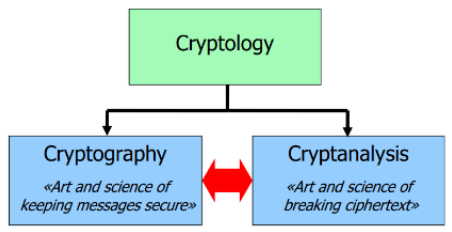
\includegraphics[width=0.6\linewidth]{its_goals.png}
\end{definition}

\begin{concept}{Business IT Risks}
\begin{itemize}
    \item Data loss
    \item System outage
    \item Espionage
    \item Sabotage
    \item Reputation loss
    \item Misuse of computing resources
    \item Violation of regulations
    \item Fraud
    \item Brand misuse
    \item Ransom demands
\end{itemize}
These risks can have significant financial, operational, and reputational impacts.
\end{concept}

\multend

\raggedcolumns

\subsubsection{Security Frameworks and Controls}

\mult{2}

\begin{concept}{Security Control Frameworks}
Security frameworks provide structured approaches to implementing security controls:
\begin{itemize}
    \item \textbf{CIS Controls} - Prioritized set of actions to protect organizations
    \item Controls are typically organized in implementation groups based on difficulty and impact
    \item Focus on preventing the most common attack vectors first
\end{itemize}
\end{concept}

\begin{definition}{Types of Security Measures}
Security measures can be categorized based on their focus:
\begin{itemize}
    \item \textbf{Preventive} - Block threats before they occur (firewalls, access controls)
    \item \textbf{Detective} - Identify when a breach has occurred (IDS, audit logs)
    \item \textbf{Corrective} - Mitigate damage after an incident (backups, incident response)
\end{itemize}
\end{definition}

\multend

\subsubsection{Disaster Recovery}



\begin{concept}{Business Continuity Management}
Disaster recovery and business continuity planning are essential for maintaining availability:
\begin{itemize}
    \item \textbf{Recovery Plan} - Detailed procedures for recovering from incidents
    \item \textbf{Recovery Tests} - Regular testing of recovery procedures
    \item \textbf{Redundancy} - Duplicate systems, power supplies, and network connections
    \item \textbf{Offline backups} - Protection against ransomware and other threats
\end{itemize}
\end{concept}

\begin{KR}{Disaster Recovery Planning}
\paragraph{Initial Assessment}
\begin{itemize}
    \item Identify critical systems and data
    \item Determine acceptable recovery time objectives (RTO)
    \item Determine acceptable recovery point objectives (RPO)
\end{itemize}

\paragraph{Plan Development}
\begin{itemize}
    \item Document recovery procedures
    \item Assign roles and responsibilities
    \item Include contact details for all relevant parties
    \item Develop technical instructions for restoration
\end{itemize}

\paragraph{Testing}
\begin{itemize}
    \item Conduct regular theoretical dry runs
    \item Perform practical tests (e.g., server shutdown, data restoration)
    \item Update procedures based on test results
\end{itemize}

\paragraph{Regular Review}
\begin{itemize}
    \item Review and update plans regularly
    \item Consider changes in infrastructure, personnel, and threats
\end{itemize}
\end{KR}

\begin{example}
A medium-sized company implements a disaster recovery plan for their customer database. They define an RTO of 4 hours and an RPO of 15 minutes, meaning they need to restore service within 4 hours with no more than 15 minutes of data loss. To achieve this, they implement a combination of hourly differential backups with continuous transaction log shipping to a standby site. Regular recovery tests are scheduled quarterly to ensure the plan remains effective.
\end{example}

\mult{2}


\begin{concept}{Problems - Overview}\\ and their impact on data availability
\paragraph{Physisch}
\textbf{unabsichtlich}
\begin{itemize}
    \item Naturkatastrophen
    \item Feuer
    \item Ausfall
    \item Kaffee auf Server
\end{itemize}

\textbf{absichtlich/bösartig}
\begin{itemize}
    \item Feuer
    \item Vandalismus
    \item Garantie läuft aus -> absichtlich langsamer
    \item Social Engineering
\end{itemize}

\paragraph{Virtuell}
\textbf{unabsichtlich}
\begin{itemize}
    \item Bitflip
    \item Config Fehler
    \item Bugs im SW
    \item Phishing klicken
\end{itemize}

\textbf{absichtlich/bösartig}
\begin{itemize}
    \item DDoS
    \item Malware
    \item Ransomware
    \item Phishing senden
    \item Trojaner
\end{itemize}
\end{concept}

\begin{theorem}{Countermeasures - Overview}

\textbf{Disaster Recovery}
    \begin{itemize}
        \item Offline backup solutions
        \item Restoring from images
    \end{itemize}

\textbf{Access Control}
    \begin{itemize}
        \item Restricted Access Rights
        \item Multi-Factor Authentication
        \item Firewalls
        \item Traffic Management Solutions
    \end{itemize}

\textbf{Physical Protection}
    \begin{itemize}
        \item Physical Access Control (locks, fences, etc.)
        \item Fire Protection (extinguishers, alarms, etc.)
        \item Monitoring (CCTV, Guards etc.)
    \end{itemize}

\textbf{Training Processes}
    \begin{itemize}
        \item Employee Training
        \item Four eyes principle
        \item Automation of routine processes
        \item Monitoring
        \item Preventive maintenance
    \end{itemize}

\textbf{Redundancy}
    \begin{itemize}
        \item Uninterruptable Power Supplies
        \item High Availability setups
        \item Load Balancing
        \item Redundant data center
        \item Redundant network connections
    \end{itemize}
\end{theorem}

\multend

\mult{2}

\begin{formula}{Recovery Plan and Test}

    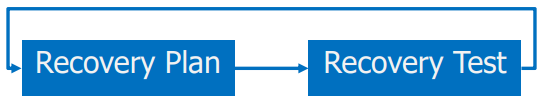
\includegraphics[width=0.7\linewidth]{recovery_plan_test.png}

    \textbf{Recovery Plan} - description of what to do if something goes wrong
    \begin{itemize}
        \item Roles and responsibilities
        \item Processes
        \item Contact details
        \item Technical instructions
    \end{itemize}

    \textbf{Recovery Test} - testing the recovery plan
    \begin{itemize}
        \item Theoretical dry run
        \item Practical tests
        \begin{itemize}
            \item turn off a server or DC
            \item restore data from backup
        \end{itemize}
    \end{itemize}
\end{formula}

\begin{concept}{Goals of IT Security}

Most measures in Information Security have one of the three following high-level goals:
\begin{itemize}
    \item Ensure data is confidential
    \item Ensure data is not corrupted
    \item Ensure data and systems are available
\end{itemize}

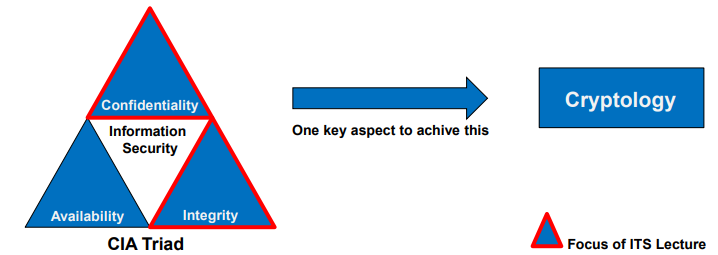
\includegraphics[width=\linewidth]{goals_of_IT_security.png}
\end{concept}

\multend

\raggedcolumns





	\raggedcolumns
	\pagebreak
	\section{Grundbegriffe und elementare Logik}

\subsection{Aussagen, Prädikate und Quantoren}

\begin{definition}{Aussage}
    `sprachliches Gebilde'' oder Ausdruck verstehen, welchem ein Wahrheitswert ``wahr'' oder ``falsch'' zugeordnet werden kann
\end{definition}

\begin{remark}
    Die Zeichenfolge ``$:=$'' steht für ``ist definiert als'' oder ``ist per Definition gleich''.
\end{remark}

\begin{remark}
    Obwohl nach Definition jede Aussage einen eindeutigen Wahrheitswert besitzt, bedeutet dies nicht, dass dieser bekannt sein muss. Der Satz ``es gibt unendlich viele Primzahlen'' war beispielsweise bereits eine Aussage, bevor man wusste, dass er wahr ist.
\end{remark}

\begin{example}
    Beispiel für eine Aussage mit Wahrheitswert: ``$3+4=106$'' (falsch)
\end{example}

\begin{example}
    Weitere Beispiele für Aussagen mit ihren Wahrheitswerten:
    \begin{enumerate}
        \item ``Jede natürliche Zahl ist entweder durch $2$ oder durch $3$ teilbar.'' (falsch)
        \item ``Es gibt unendlich viele natürliche Zahlen.'' (wahr)
    \end{enumerate}
\end{example}

\begin{definition}{Freie Variable}
    Wir sagen, dass $x$ als eine freie Variable in einem Ausdruck $A$ vorkommt, falls $x$ einen reinen Platzhalter darstellt (steht weder für einen noch für eine Menge von konkreten Werten). Beispiele: ``$x<3$'' oder ``$x$ ist ein Tisch''
    \\ Im Gegensatz dazu kommt $x$ in ``alle $x$, die durch $4$ teilbar sind, sind gerade'' nicht frei vor, weil in dieser Aussage die Gesamtheit (Menge) aller möglichen Belegungen von $x$ betrachtet wird.
\end{definition}

\begin{remark}
    In einem Ausdruck können beliebig viele Variablen frei vorkommen und wir schreiben $A(x,y,z,\dots)$, um anzuzeigen, dass in einem Ausdruck $A$ die Variablen $x,y,z,\dots$ frei vorkommen.
\end{remark}

\begin{definition}{$n$-stelliges Prädikat}
    Es sei $n$ eine natürliche Zahl. Ein Ausdruck, in dem $n$ viele Variablen frei vorkommen und der bei Belegung aller freien Variablen in eine Aussage übergeht, nennen wir ein $n$-stelliges Prädikat. Aussagen sind $0$-stellige Prädikate.
\end{definition}

\begin{remark}
    Ist $A(x)$ ein Prädikat und ist $y$ ein mathematisches Objekt (z.B. $y=17$) so, dass $A(y)$ eine wahre Aussage ist, dann sagen wir, dass das Prädikat (manchmal auch die Eigenschaft) $A$ auf $y$ zutrifft. Das Prädikat $x>100$ trifft zum Beispiel auf die Zahl $232$ zu, weil $232>100$ eine wahre Aussage ist.
\end{remark}

\begin{example}
    Beispiele für Prädikate:
    \begin{enumerate}
        \item $P(p):= $\,``$p$ ist eine Primzahl.''
        \item $T(x):= $\,``$x$ ist eine durch $21$ teilbare ganze Zahl.''
        \item $G(r):= $\,``$r>0$''
        \item $Q(x,y):= $\,``$x^2+14x-15=y$''
    \end{enumerate}
    Die Aussagen
    \begin{align*}
        &T(42)& 	    &P(7)&		&Q(2,17)&\\
        &T(357)&  &P(2)& 	&Q(1,0)&
    \end{align*}
    sind alle wahr. Deshalb können wir, entsprechend der vorhergehenden Bemerkung, z.B. ``$T$ trifft auf $42$'' zu oder auch ``$7$ hat die Eigenschaft $P$'' sagen.
\end{example}

\begin{example}
    Weitere Beispiele für Prädikate:
    \begin{itemize}
        \item $A(x,y) := x + y < 10$ ist ein zweistelliges Pädikat mit den freien Variablen $x$ und $y$.
        \item $B(x,y,z) := x + y < z$ ist ein dreistelliges Prädikat.
        \item Wenn wir die Variable $z$ in $B$ mit dem Wert $10$ belegen, dann erhalten wir das zweistellige Prädikat $B(x,y,10)$, welches gleichbedeutend mit dem Prädikat $A$ ist.
    \end{itemize}
\end{example}

\subsubsection{Junktoren}

\begin{concept}{Junktoren}
    Es seien $A$ und $B$ beliebige Prädikate. Wir führen folgende abkürzende Schreibweisen ein:
    \begin{itemize}
        \item $\neg A$ (gesprochen: Nicht $A$) ist das Prädikat, welches (für jede Belegung) genau dann wahr ist, wenn $A$ falsch ist.
        \item $A\wedge B$ (gesprochen: $A$ und $B$)  ist das Prädikat, welches (für jede Belegung) genau dann wahr ist, wenn sowohl $A$ als auch $B$ wahr sind.
        \item $A\vee B$ (gesprochen: $A$ oder $B$)  ist das Prädikat, welches (für jede Belegung) genau dann wahr ist, wenn $A$ wahr ist oder $B$ wahr ist (oder beide wahr sind).
        \item $A\Rightarrow B$ (gesprochen: $A$ impliziert $B$) ist das Prädikat, welches (für jede Belegung) genau dann wahr ist, wenn $\neg A\vee B$ wahr ist.
        \item $A\Leftrightarrow B$ (gesprochen: $A$ äquivalent $B$)  ist das Prädikat, welches (für jede Belegung) genau dann wahr ist, wenn $A\Rightarrow B$ und $B\Rightarrow A$ wahr sind.
    \end{itemize}
    Die Zeichen $\neg,\Rightarrow,\wedge$ und $\vee$ nennen wir \textit{Junktoren}.
\end{concept}

\begin{remark}
    Das Prädikat $A\Rightarrow B$ besagt, dass in jedem Fall in dem $A$ wahr ist auch $B$ wahr sein muss.
    Die Äquivalenz zweier Prädikate besagt also, dass diese stets denselben Wahrheitswert haben. Umgangssprachlich wird oft vorausgesetzt, dass zwischen den Prädikaten $A$ und $B$ ein ``inhaltlicher Zusammenhang'' bestehen muss, damit $A\Rightarrow B$ gelten kann. Dies ist in der mathematischen Logik nicht der Fall. Die Aussagen
    \begin{align*}
        \textit{Es gibt Einhörner}\Rightarrow 8\textit{ ist eine Primzahl}
    \end{align*}
    und
    \begin{align*}
        \textit{Spinat ist grün}\Rightarrow 2\textit{ ist eine Primzahl}
    \end{align*}
    sind beispielsweise beide (mathematisch gesehen) wahr.
\end{remark}

\begin{lemma}{Junktorenregeln}
    Seien $A,B$ und $C$ beliebige Aussagen. Es gelten folgende Äquivalenzen:\\ \\
    \begin{tabular}{lc}
        Doppelte Negation:  & $\neg\neg A\Leftrightarrow A$\\
        Kommutativität:     & $ A\wedge B\Leftrightarrow B\wedge A$\\
                            & $A\vee B\Leftrightarrow B\vee A$\\
        Assoziativität:     & $(A\wedge B)\wedge C\Leftrightarrow A\wedge (B\wedge C)$\\
                            & $(A\vee B)\vee C\Leftrightarrow A\vee (B\vee C)$\\
        Distributivität:    & $A\wedge (B\vee C)\Leftrightarrow (A\wedge B)\vee (A\wedge C)$\\
                            & $A\vee (B\wedge C)\Leftrightarrow (A\vee B)\wedge (A\vee C)$\\
        De Morgan:          & $\neg(A\wedge B)\Leftrightarrow\neg A\vee\neg B$\\
                            & $\neg(A\vee B)\Leftrightarrow \neg A\wedge\neg B$\\
        Kontraposition:     & $A\Rightarrow B\Leftrightarrow \neg B\Rightarrow \neg A$
    \end{tabular}
\end{lemma}

\begin{example}{Kontraposition}
    Wir können die eben aufgestellten Rechenregeln dazu verwenden um wiederum neue Tatsachen abzuleiten. Unter anderem folgt daraus das sogenannte Prinzip der \textit{Kontraposition}. Dieses Prinzip besagt, dass $A\Rightarrow B$ äquivalent ist zu $\neg B\Rightarrow\neg A$. Wollen wir dies nun mit unseren Rechenregeln nachvollziehen, so beginnen wir mit $A\Rightarrow B$ und wenden nacheinander verschiedene Regeln an um schlussendlich $\neg B\Rightarrow \neg A$ zu erhalten:
    \begin{align*}
                         &A\Rightarrow B\\
       \Leftrightarrow\, &\neg A\lor B                  &(\text{Definition von }A\Rightarrow B)\\
       \Leftrightarrow\, &B\lor \neg A                  &(\text{Kommutativität})\\
       \Leftrightarrow\, &\neg\neg B\lor\neg A          &(\text{Doppelte Negation})\\
       \Leftrightarrow\, &\neg B\Rightarrow \neg A      &(\text{Definition von }\neg B\Rightarrow\neg A)
    \end{align*}
\end{example}

\subsubsection{Quantoren}

\begin{concept}{Quantoren}
    Es sei $M$ eine Menge. Ist $A(x)$ ein Prädikat, dann können wie folgt neue Prädikate geformt werden:
    \begin{itemize}
        \item $\forall x\,A(x)$ (gesprochen: Für alle $x$ gilt $A(x)$) trifft genau dann zu, wenn $A$ auf jedes (mathematische) Objekt zutrifft.
        \item $\exists x\,A(x)$ (gesprochen: Es gibt ein $x$ mit $A(x)$) trifft genau dann zu, wenn es (mindestens) ein  Objekt gibt, auf welches $A$ zutrifft.
    \end{itemize}
    Die Symbole $\forall$ und $\exists$ heissen \textit{Allquantor} und \textit{Existenzquantor}.
\end{concept}

\begin{remark}
    In mathematischen Texten werden Prädikate von der Form $\exists x\,A(x)$ oft als ``es gibt \textbf{mindestens} ein $x$ mit $A(x)$'' ausgedrückt. Diese Ausdrucksform ist inhaltliche gleichbedeutend mit ``es gibt ein $x$ mit $A(x)$''. Auch in diesem Text werden wir beide sprechweisen synonym verwenden.
\end{remark}

\begin{remark}
    Ein $n$-stelliges Prädikat wird durch Quantifizierung (einer freien Variable) zu einem neuen $n-1$ stelligen Prädikat.
\end{remark}

\begin{lemma}{Quantorenregeln}
    Ist $A(x)$ ein Prädikat und $K$ eine Menge, so gelten folgende Äquivalenzen:
    \begin{enumerate}
        \item Vertauschungsregel für unbeschränkte Quantoren
            $$
                \forall x\, A(x)\Leftrightarrow \neg\exists x\,\neg A(x)
            $$
        \item Vertauschungsregel für beschränkte Quantoren
            $$
                \forall x\in K \;A(x)\Leftrightarrow \neg\exists x\in K\;\neg A(x)
            $$
        \item Beschränkter und unbeschränkter Allquantor
            $$
                \forall x\in K\;A(x)\Leftrightarrow \forall x(x\in K\Rightarrow A(x))
            $$
        \item Beschränkter und unbeschränkter Existenzquantor
            $$
                \exists x\in K\; A(x)\Leftrightarrow \exists x(x\in K\wedge A(x))
            $$
    \end{enumerate}
\end{lemma}

\begin{remark}
    Wir haben keine Distributionsregel mit Quantoren und Junktoren. Die Äquivalenzen
    $$
        \forall x\, A(x)\,\lor\,\forall x B(x)\,\Leftrightarrow\, \forall x\,(A(x)\,\lor\, B(x))
    $$
    und
    $$
        \exists x A(x)\wedge\exists x B(x)\Leftrightarrow \exists x (A(x)\wedge B(x))
    $$
    gelten im Allgemeinen \textbf{nicht}.

    Wir betrachten dazu als Gegenbeispiel die Aussagen
    $$
        A(x):=``x \text{ ist eine gerade natürliche Zahl''}
    $$
    und
    $$
        B(x):=``x\text{ ist eine ungerade natürliche Zahl''}.
    $$
    Die Aussage
    $$
        \exists x A(x)\wedge\exists x B(x)
    $$
    besagt also in diesem Fall, dass es mindestens eine gerade natürliche Zahl gibt und dass es ebenfalls mindestens eine ungerade natürliche Zahl gibt. Diese Aussage ist offensichtlich wahr. Die Aussage
    $$
        \exists x (A(x)\wedge B(x))
    $$
    besagt nun aber, dass es eine natürliche Zahl gibt, welche ``gleichzeitig'' gerade und ungerade ist, was offensichtlich falsch ist. Die beiden Aussagen sind also nicht äquivalent.
\end{remark}

\begin{example}
    Einige quantifizierte Aussagen mit ihren Wahrheitswerten:
    \begin{enumerate}
        \item Es sei $S$ die Menge aller Schweine und $R(x)$ das Prädikat ``$x$ ist rosa''. Es gilt
            $$
                \text{``}\exists x\in S\; R(x)\text{''}\Leftrightarrow\text{``es gibt rosa Schweine''}.
            $$
            Diese Aussage ist offensichtlich wahr. Wenn wir nun die Allquantifizierung betrachten, so erhalten wir
            $$
                \text{``}\forall x\in S\; R(x)\text{''}\Leftrightarrow\text{``alle Schweine sind rosa''}.
            $$
            Dies ist eine falsche Aussage, da etwa Wildschweine einerseits Elemente von $S$ sind aber andererseits $R$ nicht erfüllen, da sie nicht rosa sind.
        \item Wir wollen nun die Aussage
            $$
                A:=``\,\text{alle Informatiker können programmieren''}
            $$
            mit Quantoren ausdrucken.
            Wir definieren dazu zuerst das Prädikat
            $$
                B(x):=``x\text{ kann programmieren''}.
            $$
            Wir haben nun zwei mögliche Vorgehensweisen. Einerseits können wir die Menge $I$ aller Informatiker betrachten und kommen dann mittels der Aussage
            $$
                \forall x\in I\;B(x)
            $$
            zum Ziel. Andererseits können wir auch $A$ umformulieren als ``alles was ein Informatiker ist kann programmieren'' und erhalten die gewünschte Aussage mit einem uneingeschränkten Quantor
            $$
                \forall x(x\in I\Rightarrow B(x)).
            $$
            Diesen Zusammenhang zwischen eingeschränkten und uneingeschränkten Quantoren werden wir in der nächsten Bemerkung zu ``Rechenregeln für Quantoren'' allgemein formulieren.
    \end{enumerate}
\end{example}

\begin{example}
    Einige geläufige Notationen und Abkürzungen im Zusammenhang mit Quantoren sind:
    \begin{itemize}
        \item $\forall x,y\,(\dots)$ als Abkürzung von $\forall x\,\forall y\, (\dots)$ und $\exists x,y\,(\dots)$ als Abkürzung für $\exists x\,\exists y\,(\dots)$. Entsprechende Abkürzungen gelten auch für drei oder mehr quantifizierte Variablen.
        \item $\exists ! x\,(\dots)$ für ``es gibt \textbf{genau} ein $x$ mit $\dots$''.
        \item $\nexists x\,(\dots)$ für $\neg\exists x\,(\dots)$.
        \item $\forall x<y\,(\dots)$ für $\forall x\,(x<y\Rightarrow \dots)$. Diese Notation wird auch für andere ähnliche Relationen wie $ >,\leq, \geq, \subseteq, $ usw. verwendet.
    \end{itemize}
\end{example}

\begin{example}
    Mit den Rechenregeln für Quantoren und den Rechenregeln für Junktoren können wir wieder neue Tatsachen (=Wahrheitswerte neuer Aussagen) herleiten. Als Beispiel betrachten wir das Duale zur Vertauschungsregel für unbeschränkte Quantoren, nämlich:
    $$
        \exists xA(x)\Leftrightarrow \neg \forall x\neg A(x)
    $$
    Wir beginnen also mit $\exists xA(x)$ und erhalten durch Anwenden der Rechenregeln $\neg \forall x\neg A(x)$.
    \begin{align*}
        &\exists xA(x)\\
        \Leftrightarrow&\neg\neg\exists xA(x)&(\text{Doppelte Negation}) \\
        \Leftrightarrow&\neg(\neg\exists x A(x))\\
        \Leftrightarrow&\neg(\neg\exists x \neg(\neg A(x)))&(\text{Doppelte Negation})\\
        \Leftrightarrow&\neg(\forall x\neg A(x))&(\text{Vertauschungsregel})
    \end{align*}
\end{example}

\begin{example}
    Gegeben sind die Aussagen $A$ und $B$:
    \begin{enumerate}
        \item[] $A$ :=``Alle Hasen haben lange Ohren.''
        \item[] $B$ := ``Es gibt Hasen mit kurzen Beinen.''
    \end{enumerate}
    \tcblower
    Es gilt:
    \begin{enumerate}
        \item $\neg A$ entspricht ``Es gibt mindestens einen Hasen, der keine langen Ohren hat.''
        \item $A\wedge \neg B$ entspricht ``Alle Hasen haben lange Ohren und keine kurzen Beine.''
        \item $A\Rightarrow B$ entspricht ``Wenn alle Hasen lange Ohren haben, dann gibt es Hasen mit kurzen Beinen.''
    \end{enumerate}
\end{example}

\begin{example}
    Negieren Sie umgangssprachlich folgende Aussagen (so präzise wie möglich).
    \begin{enumerate}
        \item Alle Autos haben vier Räder.
        \item Zwillinge haben stets die identische Haarfarbe.
        \item Es gibt flugunfähige Vögel.
        \item Alle Dinosaurier sind ausgestorben.
    \end{enumerate}
    \tcblower
    \begin{enumerate}
        \item Es gibt ein Auto, das nicht vier Räder hat.
        \\ \textbf{Anmerkung:} Es kann auch mehrere solche Autos geben.
        \item Es gibt ein Zwillingspaar mit verschiedenen Haarfarben.
        \item Alle Vögel sind flugfähig.
        \item Mindestens ein Dinosaurier lebt noch.
    \end{enumerate}
\end{example}

\begin{example}
    Es seien $P(x)$ ein einstelliges und $Q(y,z)$ ein zweistelliges Prädikat. Formalisieren Sie:
    \begin{enumerate}
        \item Es gibt genau ein $x$ mit $P(x)$.
        \item Es gibt mindestens zwei Dinge mit der Eigenschaft $P$.
        \item Es gibt höchstens ein $x$ mit $P(x)$.
        \item Wenn $P(x)$ und $P(y)$ gilt, dann gilt stets auch $Q(x,y)$.
        \item Für kein $x$ gilt $Q(x,x)$.
    \end{enumerate}
    \tcblower
    Mögliche Lösungen:
    \begin{enumerate}
        \item $\exists x\,(P(x))\,\land\, \forall y,z\, (P(y)\land P(z)\,\Rightarrow\, y=z)$
        \item $\exists x,y\,(P(x)\land P(y)\land x\neq y)$
        \item $\neg \exists x,y\,(P(x)\land P(y)\land x\neq y)$
        \item $\forall x,y\,(P(x)\land P(y)\,\Rightarrow Q(x,y))$
        \item $\forall x\,\neg Q(x,x)$
    \end{enumerate}
\end{example}

\begin{example}
    Geben Sie Prädikate $P(x)$ und $Q(x)$ an, so dass $\forall x\,P(x)\,\lor\,\forall x\,Q(x)$ falsch, aber $\forall x\,(Q(x)\,\lor\, P(x))$ wahr ist.
    \tcblower
    Zum Beispiel:
    $$
        P(x):= x>10
    $$
    und
    $$
        Q(x):= x<11.
    $$
    Die Aussage $\forall x\, P(x)\lor \forall x\,Q(x)$ bedeutet, dass jede Zahl grösser als Zehn ist oder, dass jede Zahl kleiner als $11$ ist, diese Aussage ist falsch. Die Aussage $\forall x\,(P(x)\lor Q(x))$ besagt hingegen wahrheitsgemäss, dass jede Zahl (für sich selbst betrachtet) entweder kleiner als $11$ oder grösser als $10$ ist.
\end{example}

\begin{example}
    Gruppieren Sie folgende Aussagen so, dass in jeder Gruppe alle Aussagen äquivalent sind und keine äquivalenten Aussagen in verschiedenen Gruppen sind.
    \begin{itemize}
        \item[1.] $\forall x\,(P(x)\Rightarrow Q(x))$
        \item[2.] $\exists x\,(P(x)\Leftrightarrow Q(x))$
        \item[3.] $\forall x\,(Q(x)\Rightarrow P(x))$
        \item[4.] $\forall x\,(\neg P(x)\Rightarrow \neg Q(x))$
        \item[5.] $\forall x\,(\neg Q(x)\Rightarrow \neg P(x))$
        \item[6.] $\neg\exists x\,(\neg \neg Q(x)\land\neg P(x) )$
        \item[7.] $\neg\exists x\,(P(x)\land\neg Q(x))$
        \item[8.] $\exists x\, (P(x)\land Q(x))\lor \exists x (\neg P(x)\land\neg Q(x))$
        \item[9.] $\forall x\,\exists y\,(P(x)\land P(y))$
    \end{itemize}
    \tcblower
    Die Aussagen $1.,\,5.,\,7.$ und $3.,\,4.,\,6.$ und $2.,8.$ sind jeweils untereinander äquivalent. Es gibt keine weiteren Äquivalenzen.
\end{example}

\subsection{Grundlegende Beweistechniken}

\begin{KR}{Direkter Beweis einer Implikation}\\
    \textbf{Problemstellung:} Es gilt eine Aussage $A\,\Rightarrow \, B$ zu beweisen.\\
    \textbf{Lösungsstrategie:} Wir geben, basierend auf der Annahme, dass $A$ wahr ist, \textit{zwingende} Argumente für die Richtigkeit von $B$.
    \tcblower
    \textbf{Beispiel:} Wir zeigen, wenn $x$ und $y$ gerade (natürliche) Zahlen sind, dann ist auch $x\cdot y$ gerade.

    Wir nehmen an $x,y$ seien (irgendwelche) gerade natürliche Zahlen (Voraussetzung). Da $x,y$ gerade sind, gibt es natürliche Zahlen $n_x$ und $n_y$ so, dass
    \begin{align*}
        x=2\cdot n_x&&y=2\cdot n_y
    \end{align*}
    gilt. Für das Produkt $x\cdot y$ gilt folglich
    $$
        x\cdot y \,=\, (2\cdot n_x)\cdot(2\cdot n_y)=2\cdot(n_x\cdot 2\cdot n_y)
    $$
    und ist somit dass $x\cdot y$ ein vielfaches von $2$ also gerade ist.
\end{KR}

\begin{KR}{Beweis durch Kontraposition}\\
    \textbf{Problemstellung:} Es gilt eine Aussage von der Form $A\Rightarrow B$ zu beweisen.\\
    \textbf{Lösungsstrategie:} Beweisen Sie die Kontraposition $\neg B\Rightarrow\neg A$.
    \tcblower
    \textbf{Beispiel:} ``Für jede natürliche Zahl $n$ gilt: $(n^2+1=1)\Rightarrow (n=0)$''

    Ist $n\neq 0$ so folgt, dass auch $n^2\neq 0$ gilt. Dies impliziert, dass für jede weitere natürliche Zahl $m$ die Ungleichung $n^2+m\neq m$ erfüllt ist. Insbesondere gilt daher, dass (der Fall $m=1$) $n^2+1\neq 1$ gilt.
\end{KR}

\begin{KR}{Beweis einer Äquivalenz}\\
    \textbf{Problemstellung:} Es gilt eine Aussage von der Form $A\Leftrightarrow B$ zu beweisen.\\
    \textbf{Lösungsstrategie:} Beweisen Sie $B\Rightarrow A$ sowie $A\Rightarrow B$.
    \tcblower
    \textbf{Beispiel:} ``Für jede natürliche Zahl $n$ gilt: $(n^2+1=1)\Leftrightarrow (n=0)$''

    Wir haben in den vorhergehenden Beispielen bereits $A\Rightarrow B$ bewiesen, wir müssen also nur noch $B\Rightarrow A$ beweisen. Wir nehmen also $B$ an, es gelte also $n=0$. Draus folgt $n^2=n\cdot n=0\cdot 0=0$ und somit $n^2+1=0+1=1$.
\end{KR}

\begin{KR}{Beweis durch Widerspruch}\\
    \textbf{Problemstellung:} Es gilt eine Aussage $A$ zu beweisen.\\
    \textbf{Lösungsstrategie:} Nehmen Sie an, die Aussage $A$ wäre falsch und benützen Sie diese Annahme um einen Widerspruch herzuleiten. Leiten Sie also unter der Annahme der Falschheit von $A$ eine Aussage her von der bereits bekannt ist, dass sie falsch ist oder im Widerspruch zur Annahme steht.
    \tcblower
    \textbf{Beispiel:} $A$:=``Es gibt keine grösste natürliche Zahl''

    Wir nehmen an, dass es eine grösste natürliche Zahl gibt, wir nennen sie $m$. Wir wissen, dass
    für jede natürliche Zahl $n$ gilt, dass einerseits $n+1$ ebenfalls eine natürliche Zahl ist und dass
    andererseits $n<n+1$ erfüllt ist. Wir wenden dies auf die natürliche Zahl $m$ an und erhalten
    damit eine grössere natürliche Zahl (nämlich $m+1$). Dies steht jedoch im
    Widerspruch zu unserer ursprünglichen Annahme, dass $m$ die grösste natürliche Zahl sei.
\end{KR}

\begin{KR}{Beweis durch (Gegen-) Beispiel}\\
    \textbf{Problemstellung:} Es gilt zu zeigen, dass eine bestimmte Eigenschaft nicht auf alle Objekte (aus einem Kontext) zutrifft.\\
    \textbf{Lösungsstrategie:} Geben Sie konkret ein Objekt an, welches die erwähnte Eigenschaft nicht besitzt.
    \tcblower
    \textbf{Beispiel:} ``Nicht jede natürliche Zahl ist eine Quadratzahl.''

    Weil die Funktion $f(x)=x^2$ monoton ist (später mehr dazu) und weil $1\cdot1<2<2\cdot2$ gilt, kann die Zahl $2$ nicht als Quadrat von einer natürlichen Zahl geschrieben werden. Somit ist $2$ das (oder ein) gesuchte Gegenbeispiel.
\end{KR}

\begin{example}
    Beweisen Sie: Jeder (ganzzahlige) Geldbetrag von mindestens $4$ Cents lässt sich allein mit Zwei- und Fünfcentstücken bezahlen.\\
    \textit{Hinweis:} Machen Sie eine Fallunterscheidung ob der zu bezahlende Betrag gerade oder ungerade ist.
    \tcblower
    Zuerst bemerken wir, dass jeder gerade Betrag mit Zweicentstücken bezahlt werden kann. Ist der gegebene Betrag, sagen wir $x$ cent, ungerade, so muss er mindestens fünf Cent entsprechen, es gilt also $x\geq 5$. Weil $x$ ungerade ist, ist $x-5$ gerade. Wie wir bereits festgestellt haben können wir diesen geraden Betrag mit lauter Zweicentstücken bezahlen. Der gesamte Betrag kann also mit einem Fünfcentstück und Zweicentstücken bezahlt werden.
\end{example}

\begin{example}
    Beweisen Sie, dass man $\sqrt{2}$ nicht als Bruch schreiben kann.\\
    \textit{Hinweis:} Wenden Sie ein Widerspruchsargument an.
    \tcblower
    Wir nehmen an, dass $\sqrt{2}$ als gekürzten Bruch dargestellt werden kann und leiten daraus einen Widerspruch her. Es seien $a,b$ ganze, teilerfremde Zahlen mit
    \begin{align*}
        \sqrt{2}=\frac{a}{b}.
    \end{align*}
    Quadrieren auf beiden Seiten ergibt
    \begin{align*}
        2=\frac{a^2}{b^2}
    \end{align*}
    und somit
    \begin{align*}
        a^2=2b^2.
    \end{align*}
    Die Zahl $a^2$ muss also gerade sein. Daraus folgt, dass auch $a$ selbst gerade ist. Weil $a$ gerade ist, gibt es eine ganze Zahl $c$ mit der Eigenschaft
    $$
        a=2c.
    $$
    Daraus folgt
    $$
        2b^2=a^2=(2c)^2=4c^2
    $$
    und damit
    $$
        b^2=2c^2.
    $$
    Anhand der letzten Gleichung sehen wir, dass $b^2$ und somit auch $b$ gerade sein muss, dies widerspricht aber der Annahme, dass die Zahlen $a$ und $b$ teilerfremd seien.
\end{example}

	\raggedcolumns
	\pagebreak
	\section{Syntax und Semantik}

\subsection{Syntax}

\begin{definition}{Alphabet der Aussagenlogik}
    Das \textit{Alphabet der Aussagenlogik} (auch Zeichenvorrat genannt) besteht aus:
    \begin{itemize}
        \item Konstanten $\top$ und $\bot$.
        \item Variablen $p,q,r,s,\dots,p_0,p_1,p_2,\dots$
        \item Klammern $(,)$
        \item Junktoren $\neg,\land,\lor,\to$
    \end{itemize}
    Die Menge der Variablen bezeichnen wir mit $\mathbb{V}$.
\end{definition}

\begin{definition}{Atomare Formel}
    Jede Variable und jede Konstante ist eine \textit{atomare Formel}. Wir bezeichnen die
    Menge aller atomaren Formeln mit $\mathbb{A}:=\{\bot,\top,p,q,r,s,\dots,p_0,p_1,p_2,\dots
    \}$.
    Die \textit{Formeln} der Aussagenlogik sind dann wie folgt gegeben:
    \begin{itemize}
        \item Alle atomaren Formeln sind Formeln.
        \item Sind $P$ und $Q$ schon Formeln, dann auch: $(P\land Q)$, $(P\lor Q)$, $(P\to Q)$ und $\neg P$.
    \end{itemize}
    Wir schreiben $\mathbb{F}$ für die Menge aller aussagenlogischen Formeln.
\end{definition}

\begin{remark}
    Ist eine Formel von einem Klammernpaar umgeben, dann lassen wir die äussersten Klammern zugunsten einer besseren Lesbarkeit weg; wir schreiben beispielsweise $(p_0\lor p_1)\land p_3$ anstelle von $((p_0\lor p_1)\land p_3)$. Des Weiteren setzen wir folgende Operatorrangfolge fest: Die Negation bindet stärker als die Konjunktion und die Disjunktion, die wiederum stärker binden als die Implikation.
\end{remark}

\begin{example}
    Einige aussagenlogische Formeln:
    \begin{align*}
        &p\lor(p\to \neg(q\land p))&&p\land\neg p&&p\to(q\to p)& &\neg(p\lor\neg q)&
    \end{align*}
    Einige Zeichenreihen, die \textit{keine} aussagenlogische Formeln sind:
    \begin{align*}
        &\neg\to p& &\forall x\,p(x)& &\text{``es regnet''}&
    \end{align*}
\end{example}

\subsection{Semantik}

\begin{definition}{Belegung}
    Eine \textit{Belegung} ist eine Zuordnung von Variablen zu Wahrheitswerten, d.h.
    eine  Funktion $B:\mathbb{V}\to \{\true,\false\}$.
\end{definition}

\begin{definition}{Formale Definition Belegung}
    Es sei eine Belegung $B$ gegeben. Die Funktion $\widehat{B}$ ist die Funktion, die jeder
    aussagenlogischen Formel ihren Wahrheitswert bezüglich der Belegung $B$ zuordnet, d.h.
    die Funktion $\widehat{B}:\mathbb{F}\to\{\false,\true\}$ ist gegeben durch:
    \begin{itemize}
        \item $\widehat{B}(\bot) =\false$ und $\widehat{B}(\top)=\true$.
        \item Für beliebige Variablen $v$ gilt $\widehat{B}(v)=B(v)$.
        \item Für beliebige Formeln $F$ und $G$ gilt:
            \begin{align}
                \widehat{B}(F\land G)&=\begin{cases}
                    \true &\text{falls }\widehat{B}(F)=\true\text{ und }\widehat{B}(G)=\true\\
                    \false&\text{sonst.}
                \end{cases}\\
                \widehat{B}(F\lor G)&=\begin{cases}
                    \true&\text{falls }\widehat{B}(F)=\true\text{ oder }\widehat{B}(G)=\true\\
                    \false&\text{sonst.}
                \end{cases}\\
                \widehat{B}(\neg F)&=\begin{cases}
                    \true&\text{falls }\widehat{B}(F)=\false \\
                    \false&\text{sonst.}
                \end{cases}\\
                \widehat{B}(F\to G)&=\widehat{B}(\neg F\lor G).
            \end{align}
    \end{itemize}
\end{definition}

\begin{remark}
    Die Junktoren können wir auch als boolesche Funktionen (Funktionen, die
    Wahrheitswerte verarbeiten) anschauen:
    \begin{align*}
        \for(x,y) &= \begin{cases}
            \true&\text{falls }x=\true\text{ oder }y=\true\\
            \false&\text{sonst}
        \end{cases}\\
        \fand(x,y) &= \begin{cases}
            \true&\text{falls }x=\true\text{ und }y=\true\\
            \false&\text{sonst}
        \end{cases}\\
        \fnot(x) &=\begin{cases}
            \true&\text{falls }x=\false\\
            \false&\text{sonst}
        \end{cases}
    \end{align*}
    Durch diese Interpretation können wir die obige Definition etwas knapper formulieren:
    \begin{itemize}
        \item $\widehat{B}(F\land G)=\fand(\widehat{B}(F),\widehat{B}(G))$
        \item $\widehat{B}(F\lor G)=\for(\widehat{B}(F),\widehat{B}(G))$
        \item $\widehat{B}(\neg F)=\fnot(\widehat{B}(F))$
    \end{itemize}
    Mithilfe dieser Darstellung können wir, wenn eine Belegung $B$ gegeben ist, den Wahrheitswert einer beliebigen aussagenlogischen Formel unter der Belegung $B$ ``berechnen''.
\end{remark}

\begin{example}
    Es sei eine Belegung $B$ gegeben, die $B(p_n)=\true$ genau dann erfüllt, wenn $n$ eine
    gerade Zahl ist. Wir berechnen den Wahrheitswert von $(p_4\to(p_5\to p_6))\lor p_{13}.$
    \tcblower
    \begin{align*}
        \widehat{B}((p_4\to(p_5\to p_6))\lor p_{13})&=\for(\widehat{B}(p_4\to(p_5\to p_6)),
        \underbrace{\widehat{B}(p_{13})}_{\false}\}\\
        &=\widehat{B}(p_4\to(p_5\to p_6))\\
        &=\widehat{B}(\neg p_4\,\lor\,(p_5\to p_6))\\
        &=\for(\widehat{B}(\neg p_4),\widehat{B}(p_5\to p_6))\\
        &=\for( \fnot(\underbrace{\widehat{B}( p_4)}_{\true}),\widehat{B}(\neg p_5\,\lor\,
        p_6))\\
        &=\for( \false,\widehat{B}(\neg p_5\,\lor\,
        p_6))\\
        &=\widehat{B}(\neg p_5\,\lor\, p_6)\\
        &=\for(\widehat{B}(\neg p_5),\underbrace{\widehat{B}(p_6)}_{\true})\\
        &=\true
    \end{align*}
\end{example}

\begin{example}
    Von einer Belegung $B:\mathbb{V}\to \{\false,\true\}$ seien folgende Werte bekannt:
    \begin{align*}
        B(p) &= B(q) = B(r) = B(s) =\true\\
        B(u) &= B(v) = \false
    \end{align*}
    Bestimmen Sie $\hat B$ von folgenden Formeln:
    \begin{enumerate}
        \item $p\to s$
        \item $(u\to r)\land s$
        \item $v\lor((r\to s)\land u)$
    \end{enumerate}
    \tcblower
    \begin{enumerate}
        \item
            \[
                \hat B(p\to s)=\hat B(\neg p\lor s)=\for(\hat B(\neg p),\underbrace{\hat
                B(s)}_{\true})=\true
            \]
        \item
            \begin{align*}
                \hat B((u\to r)\land s)&=\fand (\hat B((u\to r)), \underbrace{\hat
                B(s)}_{\true})=\hat B(u\to r)\\
                &=\hat B(\neg u\lor r)=\for(\hat B(\neg u),\underbrace{\hat B(r)}_{\true})=\true
            \end{align*}
        \item
            \begin{align*}
                \hat B(v\lor((r\to s)\land u))
                &=\for(\underbrace{\hat B(v)}_{\false},\hat B((r\to s)\land u))\\
                &=\hat B((r\to s)\land u)\\
                &=\fand(\hat B(r\to s),\underbrace{\hat B(u)}_{\false})=\false
            \end{align*}
    \end{enumerate}
\end{example}

\subsubsection{Wahrheitstabellen}

\begin{definition}{Teilformel}
    Der Begriff einer \textit{Teilformel} einer Formel $F$ ist wie folgt gegeben:
    \begin{itemize}
        \item Wenn $F$ eine atomare Formel ist, dann ist besitzt $F$ nur die Teilformel $F$ (also ``sich selbst'').
        \item Wenn $F$ von der Form $A\lor B$, $A\land B$ oder $A\to B$ ist, dann besitzt $F$ als Teilformeln, neben $F$ selbst, alle Teilformeln von $A$ und $B$.
        \item Wenn $F$ von der Form $\neg A$ ist, dann besitzt $F$ als Teilformeln, neben $F$ selbst, alle Teilformeln von $A$.
    \end{itemize}
    Eine \textit{echte} Teilformel einer Formel $F$ ist eine von $F$ verschiedene Teilformel von $F$.
\end{definition}

\begin{example}
    Die Teilformeln der Formel $r\to (s\land p)$ sind $r,s,p,s\land p$ sowie $r\to (s\land p)$.
\end{example}

\begin{example}
    Die Teilformeln von der Formel $p_0\to (q\lor p_1)$ sind: $p_0,p_1,q,(q\lor p_1)$ und $p_0\to (q\lor p_1)$.
\end{example}

\begin{definition}{Wahrheitstabelle}
    In einer \textit{Wahrheitstabelle einer Formel} $F$ entspricht jede Spalte einer Teilformel von $F$ und jede Zeile einer Belegung der in $F$ vorkommenden Variablen. Es gelten folgende Bedingungen:
    \begin{itemize}
        \item In der Spalte einer Formel steht in jeder der folgenden Zeilen der Wahrheitswert dieser Formel unter der der Zeile entsprechenden Belegung.
        \item Steht in einer Spalte eine Formel, dann kommen alle echten Teilformeln dieser Formel in Spalten weiter links vor.
        \item Der letzte Eintrag der ersten Zeile ist die Formel $F$.
    \end{itemize}
\end{definition}

\begin{example}
    Eine vollständige Wahrheitstabelle von $p_0\to (q\lor p_1)$ ist:
    \begin{center}
        \begin{tabular} {| c | c | c || c | c |}
            \hline
            $p_0$ & $q$ & $p_1$ & $q\lor p_1$ & $p_0\to (q\lor p_1)$ \\ \hline
            0 & 0 & 0 & 0 & 1 \\
            0 & 0 & 1 & 1 & 1\\
            0 & 1 & 0 & 1 & 1\\
            0 & 1 & 1 & 1& 1\\
            1 & 0 & 0 & 0 & 0\\
            1 & 0 & 1 & 1 & 1\\
            1 & 1 & 0 & 1 & 1\\
            1 & 1 & 1 & 1 & 1\\ \hline
        \end{tabular}
    \end{center}
\end{example}

\subsubsection{Semantische Eigenschaften}

\begin{definition}{Wahrheitswert aussagenlogischer Formeln}
    Eine aussagenlogische Formel $A$ heisst
    \begin{itemize}
        \item \textit{Gültig} oder \textit{wahr} unter einer Belegung $B$, falls $\widehat{B}(A)=\true$.
        \item \textit{Allgemeingültig}, wenn sie unter jeder Belegung gültig ist.
        \item \textit{Widerlegbar}, wenn es mindestens eine Belegung gibt, unter der $A$ nicht gültig ist.
        \item \textit{Erfüllbar}, wenn es mindestens eine Belegung gibt, unter der $A$ gültig ist.
        \item \textit{Unerfüllbar}, wenn $A$ nicht erfüllbar ist.
    \end{itemize}
\end{definition}

\begin{remark}
    Eines der grössten ungelösten Probleme der (theoretischen) Informatik ist die Frage,
    ob es einen ``effizienten'' Algorithmus gibt, der von jeder aussagenlogischen Formel
    entscheidet, ob sie erfüllbar ist oder nicht. Diese Problemstellung wird mit $\mathsf{SAT}$ (von
    engl. \textbf{sat}isfiability) bezeichnet. Die Relevanz dieser Frage kommt daher, dass sich das
    $\mathsf{P}\stackrel{?}{=}\mathsf{NP}$ Problem (die Frage, ob zwei der wichtigsten Komplexitätsklassen übereinstimmen) darauf reduzieren lässt.
\end{remark}

\begin{example}
    Einige allgemeingültige Formeln:
    \begin{align*}
        &p\lor\neg p& &p\to (q\to p)& &F\to F&.
    \end{align*}
    Einige erfüllbare  nicht allgemeingültige Formeln:
    \begin{align*}
        &p_1\lor (p_2\lor p_3)& &p_3& &p\to q&
    \end{align*}
    Einige unerfüllbare Formeln:
    \begin{align*}
        &(p_1\to\neg p_1)\land(\neg p_1\to p_1)& &\neg p_3\land p_3& &\neg (F\to F)&
    \end{align*}
    Welche der Formeln
    \begin{align*}
        &(p_1\to (p_2\lor p_1))\lor(\neg p_1\lor (p_2\land p_1))& &\neg p_3\land p_3& &\neg (F\to \neg F)&
    \end{align*}
    sind allgemeingültig, welche erfüllbar und welche unerfüllbar?
\end{example}

\begin{example}
    Zeigen Sie: Eine aussagenlogische Formel $F$ ist genau dann allgemeingültig, wenn $\neg F$ unerfüllbar ist.
    \tcblower
    Es sei $F$ eine beliebige aussagenlogische Formel. Wir müssen folgende Behauptungen beweisen:
    \begin{itemize}
        \item Ist $F$ allgemeingültig, dann ist $\neg F$ nicht erfüllbar.
        \item Ist $\neg F$ nicht erfüllbar, dann ist $F$ allgemeingültig.
    \end{itemize}
    Für die erste Behauptung nehmen wir an, dass $F$ allgemeingültig sei. Aus der Allgemeingültigkeit von $F$ folgt $\hat B(F)=\true$ für jede Belegung $B$. Somit gilt $\hat B(\neg F)=\false$ für jede Belegung $B$, also ist die Formel $\neg F$ unerfüllbar.

    Für die zweite Behauptung nehmen wir nun an, dass die Formel $\neg F$ nicht erfüllbar sei. Es gilt somit $\hat B(\neg F)=\false$ für jede Belegung $B$. Daraus folgt $\hat B(F)=\true$ für jede Belegung $B$ und somit, dass $F$ allgemeingültig ist.
\end{example}

\begin{example}
    Ist die Behauptung korrekt, dass jede Formel genau dann erfüllbar ist, wenn ihre Negation nicht erfüllbar ist? Begründen Sie Ihre Antwort.
    \tcblower
    Die Behauptung ist falsch. Ein Gegenbeispiel zu der Aussage ist die (atomare) Formel $p$, sie ist erfüllbar und die Negation $\neg p$ ist ebenfalls erfüllbar.
\end{example}

\begin{example}
    Geben Sie zwei erfüllbare Formeln $F$ und $G$ an, so dass die Formel $F\land G$ nicht erfüllbar ist.
    \tcblower
    Die Formeln $F:=p$ und $G:=\neg p$ sind beide erfüllbar, die Formel $p\land \neg p$ ist jedoch unerfüllbar.
\end{example}

\begin{definition}{Konsequenz und Äquivalenz}
    Es seien $F$ und $G$ beliebige aussagenlogische Formeln. Wir sagen
    \begin{itemize}
        \item $F$ \textit{ist eine Konsequenz von }$G$, falls $F$ unter jeder Belegung wahr ist unter der $G$ wahr ist.
        \item $F$ und $G$ sind \textit{logisch äquivalent}, wenn $G$ und $F$ unter jeder Belegung denselben Wahrheitswert annehmen.
    \end{itemize}
    Sind $F$ und $G$ äquivalente Formeln, dann schreiben wir $F\equiv G$.
\end{definition}

\begin{remark}
    Zwei aussagenlogische Formeln sind genau dann äquivalent, wenn beide Formeln von der jeweils anderen eine Konsequenz sind.
\end{remark}

\begin{lemma}{Regeln der Aussagenlogik}
    Sind $F,G$ und $H$ beliebige aussagenlogische Formeln, dann gelten folgende Äquivalenzen:
    \begin{itemize}
        \item Gesetz der doppelten Negation: $\neg\neg F\,\equiv\, F$
        \item Absorption: $F\land F\,\equiv\, F$ und $F\lor F\,\equiv\, F$
        \item Kommutativität: $F\land G\,\equiv\,G\land F$ und $F\lor G\,\equiv\, G\lor F$
        \item Assoziativität: $F\land(G\land H)\,\equiv\,(F\land G)\land H$
        \item Assoziativität: $F\lor(G\lor H)\,\equiv\,(F\lor G)\lor H$
        \item Distributivität: $F\land(G\lor H)\,\equiv\,(F\land G)\lor (F\land H)$
        \item Distributivität: $F\lor(G\land H)\,\equiv\,(F\lor G)\land (F\lor H)$
        \item De Morgan: $\neg (F\land G)\,\equiv\,\neg F\lor\neg G$
        \item De Morgan: $\neg (F\lor G)\,\equiv\,\neg F\land \neg G$
        \item Kontraposition: $F\to G\,\equiv\neg G\to\neg F$
    \end{itemize}
\end{lemma}

\begin{howto}{Äquivalenz zeigen}
    Wir müssen für jede der behaupteten Äquivalenzen nachweisen, dass die genannten Formeln unter jeder Belegung denselben Wahrheitswert haben. Wenn wir also von einer beliebigen Belegung $B$ ausgehen, dann müssen wir, um eine Äquivalenz von der Form $X\equiv Y$ nachzuweisen, bloss zeigen, dass $\widehat{B}(X)=\widehat{B}(Y)$ gilt.
    \begin{itemize}
        \item Doppelte Negation folgt aus $\fnot(\fnot(x))=x$:
            \begin{align*}
                \widehat{B}(\neg\neg F)=\fnot(\widehat{B}(\neg F))=\fnot(\fnot(\widehat{B}(F))=\widehat{B}(F).
            \end{align*}
        \item Absorbtion folgt sofort aus $\fand(x,x)=\for(x,x) =x$.
        \item Kommutativität folgt sofort aus $\for(x,y)=\for(y,x)$ und $\fand(x,y)=\fand(y,x)$.
        \item Für Assoziativität, Distributivität und DeMorgan siehe Fallunterscheidung an der Tafel.
    \end{itemize}
\end{howto}

\begin{example}
    Zeigen Sie mit der Methode der Wahrheitstabellen, dass die Formeln $p\to q$ und $q\to p$ nicht äquivalent sind.
    \tcblower
    \begin{center}
        \begin{tabular} {|c|c||c|c|}
            \hline
            $p$ & $q$ & $p\to q$ & $q \to p$ \\
            \hline
            0 & 0 & 1 & 1\\
            0 & 1 & \colorbox{red}{1} & \colorbox{red}{0}\\
            1 & 0 & \colorbox{red}{0} & \colorbox{red}{1}\\
            1 & 1 & 1 & 1\\
            \hline
        \end{tabular}
    \end{center}
\end{example}

\begin{theorem}{Folgerungstheorem}
    Sind $F$ und $G$ aussagenlogische Formeln, dann gelten:
    \begin{enumerate}
        \item[i)] $G$ ist genau dann eine Konsequenz von $F$, wenn die Formel $F\to G$ allgemeingültig ist.
        \item[ii)] $F$ und $G$ sind genau dann logisch äquivalent, wenn die Formel $F\to G\land G\to F$ allgemeingültig ist.
    \end{enumerate}
\end{theorem}

\begin{howto}{Allgemeingültigkeit zeigen}\\
    Wir behandeln zuerst die Behauptung $i)$ des Folgerungstheorems.
    \begin{align*}
        F\to G\text{ allgemeingültig } &\Leftrightarrow \forall B(\widehat{B}(F\to G) =\true)\\
        &\Leftrightarrow \forall B(\widehat{B}(\neg F\lor G) =\true)\\
        &\Leftrightarrow \forall B((\neg \widehat{B}(F)=\true) \lor (\widehat{B}(G) =\true))\\
        &\Leftrightarrow \forall B(\widehat{B}(F)=\true\Rightarrow \widehat{B}(G)=\true)\\
        &\Leftrightarrow G\text{ ist Konsequenz von }F
    \end{align*}
    Die Behauptung $ii)$ folgt direkt aus dem ersten Teil.
\end{howto}

\subsubsection{Normalformen}

\begin{definition}{Literale}
    \textit{Literale} sind atomare Formeln oder negierte atomare Formeln.
\end{definition}

\begin{example}
    Beispiele für Literale: $p$, $\neg q$, $\neg p_{34}$.
\end{example}

\begin{concept}{Normalformen}
    Eine aussagenlogische Formel ist:
    \begin{itemize}
        \item In \textit{Negationsnormalform}(NNF), wenn alle Negationen in Literalen vorkommen und wenn keine Implikationen ($\to$) vorkommen.
        \item In \textit{disjunktiver Normalform}(DNF), wenn sie von der Form
            \[
                (L_{1,1}\land L_{1,2}\land\dots)\lor(L_{2,1}\land L_{2,2}\land\dots)\lor(L_{3,1}\land L_{3,2}\land\dots)\dots
            \]
            mit Literalen $L_{i,j}$ ist.
        \item In \textit{konjunktiver Normalform}(KNF), wenn sie von der Form
            \[
                (L_{1,1}\lor L_{1,2}\lor\dots)\land(L_{2,1}\lor L_{2,2}\lor\dots)\land(L_{3,1}\lor L_{3,2}\lor\dots)\dots
            \]
            mit Literalen $L_{i,j}$ ist.
    \end{itemize}
\end{concept}

\begin{example}
    Die Formel
    \[
        \neg(p\lor q)
    \]
    ist in keiner der oben eingeführten Normalformen. Die Formel
    \[
        (\neg p\lor q)\land ((p\land p_1)\lor(p_2\land p_3))
    \]
    ist in $NNF$ aber weder in $DNF$ noch in $KNF$. Die Formel
    \[
        p\lor q
    \]
    ist in $NNF$, $KNF$ und $DNF$.
\end{example}

\begin{lemma}{Äquivalente Normalformen}
    Für jede aussagenlogische Formel gibt es äquivalente Formeln in $NNF$, $KNF$ und $DNF$.
\end{lemma}

\begin{howto}{Normalformen konstruieren}
    \begin{itemize}
        \item $NNF$: Wir gehen folgendermassen vor, um aus einer Formel eine äquivalente Formel in $NNF$ zu konstruieren.
            \begin{enumerate}
                \item[1.] Implikationen eliminieren durch Anwenden der Regel $F\to G\,\equiv\,\neg F\lor G$.
                \item[2.] Negationen, die nicht zu einem Literal gehören, werden sukzessive durch Anwenden der De Morganschen Regeln und der Regel über doppelte Negation eliminiert.
            \end{enumerate}
        \item $KNF/DNF$: Jede Formel in $NNF$ kann durch sukzessives Anwenden der Distributivgesetze wahlweise in $KNF$ oder $DNF$ gebracht werden. Da wir bereits wissen, dass jede Formel in $NNF$ gebracht werden kann, ist die Behauptung somit bewiesen.
    \end{itemize}
\end{howto}

\begin{example}
    Wir bringen die Formel
    \[
        (\neg p\to q)\to ((p\land p_1)\lor(p_2\land p_3))
    \]
    in $DNF$.
    \tcblower
    Wir eliminieren zuerst alle Implikationen und doppelten Negationen:
    \begin{align*}
        (\neg p\to q)\textcolor{red}{\to} ((p\land p_1)\lor(p_2\land p_3))\,&\equiv\, \neg(\neg p\textcolor{red}{\to} q)\lor ((p\land p_1)\lor(p_2\land p_3))\\
        &\equiv\, \neg(\textcolor{red}{\neg\neg} p \lor q)\lor ((p\land p_1)\lor(p_2\land p_3))\\
        &\equiv \neg(p \lor q)\lor ((p\land p_1)\lor(p_2\land p_3)).
    \end{align*}
    Als Nächstes eliminieren wir alle Negationen, die nicht in Literalen vorkommen:
    \begin{align*}
        \textcolor{red}{\neg(p \lor q)}\lor ((p\land p_1)\lor(p_2\land p_3))\,&\equiv\,(\neg p\land\neg q)\lor ((p\land p_1)\lor(p_2\land p_3)).
    \end{align*}
    Die Formel, die wir erhalten haben, ist sowohl in $NNF$ als auch in $DNF$. Wir konstruieren nun noch eine zur Formel
    \[
        (p\land p_1)\lor(p_2\land p_3)
    \]
    äquivalente Formel in $KNF$. Wir wenden sukzessive die Distributivgesetze an:
    \begin{align*}
        (p\land p_1)\textcolor{red}{\lor}(p_2\land p_3)&\,\equiv\,\big( (p\land p_1)\lor p_2)\land (\textcolor{red}{(p\land p_1)\lor p_3})\\
        &\equiv\, (\textcolor{red}{(p\land p_1)\lor p_2})\land ((p\lor p_3)\land(p_1\lor p_3))\\
        &\equiv\, ((p\lor p_2)\land(p_1\lor p_2))\land ((p\lor p_3)\land(p_1\lor p_3)).
    \end{align*}
\end{example}

\begin{example}
    Bringen Sie die Formel
    \[
        (p_1\to p_3)\lor(p_1\land p_2)
    \]
    in $KNF$ und in $DNF$.
    \tcblower
    \begin{align*}
        (p_1\to p_3)\lor(p_1\land p_2)&\equiv \underbrace{(\neg p_1\lor p_3)\lor (p_1\land p_2)}_{DNF}\\
        &\equiv \underbrace{((\neg p_1\lor p_3)\lor p_1)\land ((\neg p_1\lor p_3)\lor p_2)}_{KNF}
    \end{align*}
\end{example}

\begin{howto}{Normalformen aus Wahrheitstabellen}\\
    Es ist auch möglich direkt aus einer Wahrheitstabelle einer gegebenen Formel $F$ eine äquivalente Formel in $KNF$ oder $DNF$ abzulesen.
    \begin{itemize}
        \item $DNF$:  Für jede Zeile, die als Resultat $\true$ liefert, wird eine Konjunktion gebildet, die alle atomaren Teilformeln dieser Zeile verknüpft, dabei werden die Teilformeln, die in dieser Zeile (Belegung) falsch sind negiert. Schliesslich werden die so gewonnenen Konjunktionen als Disjunktion zusammengenommen.
        \item $KNF$: lässt sich dadurch konstruieren, dass man vorerst eine zu $\neg F$ äquivalente Formel in $DNF$ findet (wie oben beschrieben), diese Formel negiert und mit den Regeln von DeMorgan die Negationen in den Term schiebt.
    \end{itemize}
\end{howto}

\begin{example}
    Beispielhaft für dieses Vorgehens, bringen wir die Formel
    \begin{align*}
        p_0\to (q\land p_1)
    \end{align*}
    in $DNF$ und $KNF$.
    \tcblower
    Zuerst erstellen wir eine Wahrheitstabelle von $p_0\to (q\land p_1)$ und markieren zu jeder relevanten Zeile das gewonnene Disjunktionsglied.
    \begin{center}
        \begin{tabular} {| c | c | c || c | c | c |}
            \hline
            $p_0$ & $q$ & $p_1$ & $q\land p_1$ & $p_0\to (q\land p_1)$ & \\
            \hline
            0 & 0 & 0 & 0 & 1 & \textcolor{red}{$\neg p_0 \land \neg q\land \neg p_1$}\\
            0 & 0 & 1 & 0 & 1 & \textcolor{red}{$\neg p_0 \land \neg q\land      p_1$}\\
            0 & 1 & 0 & 0 & 1 & \textcolor{red}{$\neg p_0 \land      q\land \neg p_1$}\\
            0 & 1 & 1 & 1 & 1 & \textcolor{red}{$\neg p_0 \land      q\land      p_1$}\\
            1 & 0 & 0 & 0 & 0 & \textcolor{red}{$-$}\\
            1 & 0 & 1 & 0 & 0 & \textcolor{red}{$-$}\\
            1 & 1 & 0 & 0 & 0 & \textcolor{red}{$-$}\\
            1 & 1 & 1 & 1 & 1 & \textcolor{red}{$     p_0 \land      q\land      p_1$}\\
            \hline
        \end{tabular}
    \end{center}
    \smallskip
    Zusammengefasst ergibt sich die folgende Formel in $DNF$:
    \begin{align*}
       (\neg p_0 \land \neg q\land \neg p_1)
       \lor (\neg p_0 \land \neg q\land      p_1)
       &\lor (\neg p_0 \land      q\land \neg p_1)
       \lor (\neg p_0 \land      q\land      p_1)\\
       &\lor      (p_0 \land      q\land      p_1).
    \end{align*}
    Zum Erstellen einer Formel in KNF, betrachten wir die Wahrheitstabelle der negierten Formel:
    \begin{center}
        \begin{tabular} {| c | c | c || c | c | c | c |}
            \hline
            $p_0$ & $q$ & $p_1$ & $q\land p_1$ & $p_0\to (q\land p_1)$ & $\neg(p_0\to (q\land p_1))$ & \\
            \hline
            0 & 0 & 0 & 0 & 1 & 0 & \textcolor{red}{$-$}\\
            0 & 0 & 1 & 0 & 1 & 0 & \textcolor{red}{$-$}\\
            0 & 1 & 0 & 0 & 1 & 0 & \textcolor{red}{$-$}\\
            0 & 1 & 1 & 1 & 1 & 0 & \textcolor{red}{$-$}\\
            1 & 0 & 0 & 0 & 0 & 1 & \textcolor{red}{$p_0 \land \neg q\land \neg p_1$}\\
            1 & 0 & 1 & 0 & 0 & 1 & \textcolor{red}{$p_0 \land \neg q\land      p_1$}\\
            1 & 1 & 0 & 0 & 0 & 1 & \textcolor{red}{$p_0 \land q\land \neg p_1$}\\
            1 & 1 & 1 & 1 & 1 & 0 & \textcolor{red}{$-$}\\
            \hline
        \end{tabular}
    \end{center}
    \smallskip
    Durch Anwendung der DeMorgan Regeln erhalten wir daraus eine passende Formel in $KNF$:
    \begin{align*}
        \neg&((p_0 \land \neg q\land \neg p_1)\lor
              (p_0 \land \neg q\land p_1)\lor
              (p_0 \land q\land \neg p_1)
            )\\
            &\equiv
              \neg(p_0 \land \neg q\land \neg p_1)\land
              \neg(p_0 \land \neg q\land p_1)\land
              \neg(p_0 \land q\land \neg p_1)\\
            &\equiv
              (\neg p_0 \lor q\lor p_1)\land
              (\neg p_0 \lor q\lor \neg p_1)\land
              (\neg p_0 \lor \neg q\lor p_1)
    \end{align*}
\end{example}

	\raggedcolumns
	\pagebreak
	\section{Mengen, Relationen und Funktionen}

\subsection{Der Mengenbegriff und grundlegende Definitionen}

\begin{concept}{Notation Mengen}
    Ist $X$ eine Menge und $y$ ein \textit{Element} von $X$, dann schreiben wir $y\in X$. Ist $y$ kein Element von $X$, dann schreiben wir $y\notin X$.
\end{concept}

\begin{remark}
    Die erste \textit{definierende Eigenschaft} von Mengen ist die Tatsache, dass jede Menge durch ihre Elemente vollständig beschrieben ist.
\end{remark}

\begin{definition}{Definierende Eigenschaft}
    Zwei Mengen sind genau dann gleich, wenn sie dieselben Elemente enthalten: Es gilt für alle Mengen $X$ und $Y$ die Äquivalenz
    \[
        X=Y\,\Leftrightarrow\,\forall z\, (z\in X\Leftrightarrow z\in Y).
    \]
\end{definition}

\begin{concept}{Explizite Schreibweise}
    Sind mathematische Objekte $x_1,\dots,x_n$ gegeben, dann schreiben wir
    \[
        \{x_1,\dots,x_n\}
    \]
    für die Menge die als Elemente genau $x_1,\dots,x_n$ hat.
\end{concept}

\begin{example}
    \begin{itemize}
        \item Die Menge $\{2,34,77\}$ enthält die drei Elemente $2$, $34$ und $77$.
        \item Die Menge $\{\,\}$ heisst \textit{leere Menge}. Die leere Menge ist die einzige Menge, die gar keine Elemente besitzt, sie wird mit $\varnothing $ bezeichnet.
    \end{itemize}
\end{example}

\begin{remark}
    Wenn keine Missverständnisse zu befürchten sind, so beschreibt man Mengen auch durch ``angedeutete'' Aufzählung ihrer Elemente. Die Menge $\mathbb{N}$ der \textit{natürlichen Zahlen} wird beispielsweise durch
    \[
        \N:=\{0,1,2,\dots\}
    \]
    beschrieben.
    Die Menge der \textit{ganzen Zahlen} wird durch
    \[
        \Z:=\{\dots, -2,-1,0,1,2\dots\}
    \]
    beschrieben.
\end{remark}

\begin{remark}
    Die Tatsache, dass Mengen durch ihre Elemente eindeutig beschrieben werden hat zur Folge, dass Mengen sehr ``unstrukturierte Datentypen'' sind, d.h. Mengen haben keine ``innere Ordnung''. Es gelten unter anderem:
    \begin{itemize}
        \item Für beliebige $z,x_1,\dots,x_n$
            \[
                z\in\{x_1,\dots x_n\}\,\Leftrightarrow\, z=x_1\lor\dots\lor z=x_n
            \]
        \item Für alle $x$
            \[
                \{x\}=\{x,x\}=\{x,x,x\}=\dots
            \]
        \item Für alle $x,y$
            \[
                \{x,y\}=\{y,x\}.
            \]
    \end{itemize}
\end{remark}

\begin{concept}{Prädikative Schreibweise}
    Ist $X$ eine Menge und ist $\mathsf{E}$ eine Eigenschaft (Prädikat), dann bezeichnen wir mit
    \[
        \big\{z\in X\mid \mathsf{E}(z)\big\}
    \]
    oder mit
    \[
        \big\{z\mid z\in X\land\mathsf{E}(z)\big\}
    \]
    die Menge aller Elemente $z$ von $X$ mit der Eigenschaft $\mathsf{E}(z)$.
\end{concept}

\begin{example}
    Die Menge aller geraden natürlichen Zahlen erhält man auch durch die prädikative Schreibweise,
    \begin{itemize}
        \item $\{n\in\N\mid n\text{ ist gerade}\}$
        \item $\{n\in\N\mid \exists z\in\N\,(n=2\cdot z)\}$
    \end{itemize}
\end{example}

\begin{concept}{Ersetzungsschreibweise}
    Ist $F$ eine Funktion und ist $X$ eine Menge, dann beinhaltet die Menge
    \[
        \big\{F(x)\mid x\in X \big\}
    \]
    alle Funktionswerte $F(x)$, die man dadurch erhalten kann, dass man ein Element $x\in X$ in $F$ einsetzt:
    \[
        \big\{F(x)\mid x\in X\big\}:=\{y\mid \exists x\in X\,(y=F(x))\}.
    \]
\end{concept}

\begin{remark}
    Ist eine Funktion $f$ und eine Menge von der Form
    \begin{align*}
        X=\{x_1,x_2,x_3,\dots\}
    \end{align*}
    gegeben, dann entspricht die Menge $\{f(x)\mid x\in X\}$ der Menge
    \begin{align*}
        \{f(x_1),f(x_2),f(x_3),\dots\}.
    \end{align*}
\end{remark}

\begin{example}
    Die Menge der geraden natürlichen Zahlen lässt sich nun mithilfe der Funktion $F(x)=2\cdot x$ als
    \[
        \{F(x)\mid x\in\N\} = \{2x\mid x\in\N\}
    \]
    schreiben.
\end{example}

\begin{definition}{Teilmengen}
    Wir schreiben $X\subseteq Y$ und sagen $X$ ist eine \textit{Teilmenge} von $Y$, wenn jedes Element von $X$ auch ein Element von $Y$ ist:
    \[
        X\subseteq Y:\,\Leftrightarrow\,\forall x\,(x\in X\Rightarrow x\in Y).
    \]
    Wir schreiben $X\subsetneq Y$ und sagen $X$ ist eine \textit{echte Teilmenge} von $Y$, falls $X$ eine von $Y$ verschiedene Teilmenge von $Y$ ist:
    \[
        X\subsetneq Y\,:\Leftrightarrow\, X\subseteq Y\land X\neq Y.
    \]
\end{definition}

\begin{example}
    \begin{itemize}
        \item Die Menge aller Hühner ist eine (echte) Teilmenge der Menge aller Vögel, weil alle Hühner Vögel sind (und weil es Vögel gibt die keine Hühner sind).
        \item Die Menge aller Primzahlen ist eine (echte) Teilmenge von $\N$.
        \item Die Menge aller Primzahlen ist \textit{keine} Teilmenge aller ungeraden Zahlen, weil die Zahl $2$ eine Primzahl aber keine ungerade Zahl ist.
    \end{itemize}
\end{example}

\begin{lemma}{Äquivalenz}\\
    Zwei Mengen $X$ und $Y$ sind gleich, wenn $X\subseteq Y$ und $Y\subseteq X$ gilt.
\end{lemma}

\begin{definition}{Potenzmenge}
    Ist $A$ eine beliebige Menge, dann bezeichnen wir mit
    \[
        \mathcal{P}(A):=\{x\mid x\subseteq A\}
    \]
    die \textit{Potenzmenge} von $A$, die genau die Teilmengen von $A$ als Elemente enthält.
\end{definition}

\begin{definition}{Schnitt- und Vereinigungsmenge}\\
    Sind $X$ und $Y$ Mengen, dann ist
    \[
        X\cup Y:=\{x\mid x\in X\lor x\in Y \}
    \]
    die \textit{Vereinigung} von $X$ mit $Y$. Die \textit{Schnittmenge} von $X$ und $Y$ ist durch
    \[
        X\cap Y:=\{x\in X\mid x\in Y \}=\{x\in Y\mid x\in X\}=\{x\mid x\in X\land x\in Y\}
    \]
    gegeben. Ist $I$ eine Menge so, dass für alle Elemente $i\in I$ auch $A_i$ eine Menge ist, und $I\neq\varnothing$, dann wird die Vereinigung resp. Schnittmenge von $\{A_i\mid i\in I\}$ genannt.
    \begin{align*}
        \bigcup_{i\in I}A_i:=\{x\mid\exists i\in I\,(x\in A_i) \} & & \bigcap_{i\in I}A_i:=\{x\mid\forall i\in I\,(x\in A_i) \}
    \end{align*}
\end{definition}

\begin{example}
    \begin{enumerate}
        \item $\N=\{n\in \N\mid n\text{ ist gerade}\}\cup \{n\in \N\mid n\text{ ist ungerade}\}$
        \item $\varnothing=\{n\in \N\mid n\text{ ist gerade}\}\cap \{n\in \N\mid n\text{ ist ungerade}\}$
        \item Sind $X_a$ und $X_b$ beliebige Mengen, dann gilt:
            \[
                X_a\cup X_b=\bigcup_{i\in\{a,b\}}X_i.
            \]
        \item Ist für jede natürliche Zahl $n$ die Menge $X_n$ als $\{0,\dots, n\}$ gegeben, dann gilt
            \[
                \bigcup_{n\in \N}X_n\,=\,\N
            \]
            und
            \[
                \bigcap_{n\in \N}X_n\,=\,\{0\}.
            \]
    \end{enumerate}
\end{example}

\begin{definition}{Komplementärmenge}\\
    Sind $X$ und $Y$ beliebige Mengen, so definieren wir als
    \[
        X\setminus Y:=\{x\in X\mid x\notin Y\}
    \]
    die Menge aller Elemente von $X$, die nicht zu $Y$ gehören. Die Menge $X\setminus Y$ nennt man ``$X$ ohne $Y$''. Ist eine ``Grundmenge'' $A$ (implizit oder explizit) vorgegeben, so bezeichnet man die Menge $A\setminus Y$ auch als ``Komplement'' oder ``Komplementärmenge'' von $X$ (relativ zu $A$).
\end{definition}

\begin{lemma}{Rechenregeln}
    Es gelten für beliebige Mengen $A,B$ und $C$ folgende Identitäten: (gleich wie Junktorenregeln)
    \begin{center}
        $A\cap A=A\text{ und }A\cup A=A$\\
        $A\cup B=B\cup A\text{ und }A\cap B=B\cap A.$\\
        $A\cap(B\cap C)=(A\cap B)\cap C\text{ und }A\cup(B\cup C)=(A\cup B)\cup C$\\
        $A\cap(B\cup C)=(A\cap B)\cup (A\cap C)\text{ und }A\cup(B\cap C)=(A\cup B)\cap (A\cup C)$\\
        $(C\backslash A)\cap (C\backslash B)=C\backslash (A\cup B)\text{ und }(C\backslash A)\cup (C\backslash B)=C\backslash (A\cap B)$
    \end{center}
    Charakterisierung der Teilmengenbeziehung:
    \[
        A\subseteq B\Leftrightarrow A\cap B= A\Leftrightarrow A\cup B=B
    \]
\end{lemma}

\begin{definition}{Disjunkte Mengen}
    Zwei Mengen $X$ und $Y$ heissen \textit{disjunkt}, falls sie keine gemeinsamen Elemente haben, d.h. falls $X\cap Y=\varnothing$ gilt. Wir sagen eine Menge $\{X_i\mid i\in I \}$ von Mengen bestehe aus \textit{paarweise disjunkten} Mengen, wenn folgendes gilt:
    \[
        \forall i,j\in I\,(i\neq j\Rightarrow X_i\cap X_j=\varnothing).
    \]
\end{definition}

\begin{definition}{Partitionen}
    Eine \textit{Partition} $P=\{P_i\mid i\in I \}$ einer Menge $A$, ist eine Menge von Teilmengen von $A$, die folgende beiden Voraussetzungen erfüllt:
    \begin{itemize}
        \item Die Elemente von $P$ sind nichtleer und paarweise disjunkt.
        \item $\bigcup_{i\in I}P_i=A$
    \end{itemize}
    Die Elemente einer Partition werden \textit{Blöcke} der Partition genannt.
\end{definition}

\subsection{Funktionen}

\begin{definition}{Tupel}
    Es sei $n>0$ eine natürliche Zahl. Ein $n$\textit{-Tupel} ist ein Term von der Form
    \[
        (x_1,\dots,x_n).
    \]
    Für beliebige Tupel gilt:
    \[
        (x_1,\dots,x_n)=(y_1,\dots y_k):\Leftrightarrow n=k\land x_1=y_1\land\dots\land y_n=x_n.
    \]
    $2$-Tupel nennen wir \textit{Paare} und $3$-Tupel \textit{Tripel}.\\
    \textit{Tupel} haben im Gegensatz zu Mengen mehr innere Struktur - die Reihenfolge und Wiederholung von Elementen sind wesentlich, sie sind gewissermassen die mathematische Entsprechung zu Listen und Arrays in der Informatik.
\end{definition}

\begin{definition}{Kartesisches Produkt}
    Die Gesamtheit aller Tupel mit Elementen aus einer oder mehreren gegebenen Mengen nennt man kartesisches Produkt.\\
    Es seien $A_1,\dots, A_n$ Mengen und $n\in\N$ mit $n>0$.
    Das \textit{kartesische Produkt} von $A_1,\dots, A_n$, ist die Menge aller $n$-Tupel mit Einträgen aus den Mengen $A_1,\dots ,A_n$:
    \begin{align*}
        \prod_{i=1}^{n}A_i=\big\{(a_1,\dots,a_n)\mid a_1\in A_1\land\dots\land a_n\in A_n \big\}.
    \end{align*}
\end{definition}

\begin{remark}
    Wir schreiben auch $A_1\times A_2\times \dots\times A_n$ für $\prod_{i=1}^nA_i$.\\ Insbesondere schreiben wir $X\times Y$ für das kartesische Produkt von zwei Mengen $X$ und $Y$, konkret heisst das:
    \[
        X\times Y:=\{(x,y)\mid x\in X\land y\in Y \}.
    \]
    Für das $n$-fache kartesisches Produkt $A\times A\times\dots\times A$ einer Menge $A$ mit sich selbst schreiben wir auch $A^n$.
\end{remark}

\begin{example}
    Die Menge der rationalen Zahlen
    \[
        \Q:=\left\{\frac{x}{y}\mid x\in \Z\land y\in\N\setminus\{0\}\right\}
    \]
    kann man als das kartesische Produkt
    \[
        \Z\times(\N\setminus\{0\})
    \]
    auffassen.
\end{example}

\begin{definition}{Relation}
    Eine $n$-stellige \textit{Relation} $R$ auf den Mengen $A_1,\dots A_n$ ist eine Menge von $n$-Tupeln aus $A_1\times\dots \times A_n$. Mit anderen Worten, die Relationen auf $A_1,\dots,A_n$ sind genau die Teilmengen
    \begin{align*}
        R\subseteq A_1\times\dots \times A_n.
    \end{align*}
    Ist $R$ eine $n$-stellige Relation und gilt $(x_1,\dots,x_n)\in R$, dann sagen wir, dass die Elemente $x_1,\dots,x_n$ zueinander in Relation $R$ stehen.
    \tcblower
    Eine $2$-stellige Relation $R\subseteq X\times Y$ heisst auch eine \textit{binäre Relation} auf den Mengen $X$ und $Y$. Ist $R$ eine binäre Relation, so schreiben wir auch $xRy$ für $(x,y)\in R$.
\end{definition}

\begin{definition}{Funktion}
    Es seien $A$ und $B$ beliebige Mengen. Eine Relation $f\subseteq A\times B$ ist eine \textit{Funktion} von $A$ nach $B$, falls:
    \begin{align*}
        \forall x\in A\exists!y\in B((x,y)\in f)
    \end{align*}
    gilt. In diesem Fall schreiben wir $f:A\to B.$
\end{definition}

\begin{concept}{Notation Funktionen}
    Im Kontext einer Funktion $f:A\to B$ verwenden wir folgende Schreibweisen und Konventionen:
    \begin{itemize}
        \item Da zu jedem $x\in A$ ein eindeutig bestimmtes Element $y\in B$ mit $(x,y)\in f$ existiert, kann dieses $y$ mit $f(x)$ bezeichnet und \textit{Funktionswert von $f$ bei $x$} genannt werden.
        \item Die Menge aller Funktionswerte $Im(f) := \{f(x)\mid x\in A \}$ wird als \textit{Bild(menge)} von $f$ bezeichnet.
        \item Die Menge $A$ nennen wir den Definitionsbereich von $f$ und schreiben dafür auch $Dom(f)$.
        \item Der Definitionsbereich ist eindeutig durch die Funktion gegeben:
            \begin{align*}
                A=Dom(f)=\{x\mid \exists y ((x,y)\in f) \}=\{x\mid \exists y (f(x)=y )\}
            \end{align*}
        \item Die Menge $B$ ist durch die Voraussetzung $f:A\to B$ nicht eindeutig bestimmt, tatsächlich gilt $f:A\to B$ für jede Menge $B$ mit $Im(f)\subseteq B$.
    \end{itemize}
\end{concept}

\begin{definition}{Injektiv}
    Eine Funktion $f$ ist genau dann \textit{injektiv}, wenn die Relation
    \begin{align*}
        f^{-1}=\{(y,x)\mid (x,y)\in f\}
    \end{align*}
    eine Funktion ist.\\
    Umgangssprachlich: Jeder Output kann nur mittels einem einzigen Inputelement erreicht werden.
\end{definition}

\begin{definition}{Umkehrfunktion}\\
    Ist $f:A\to B$ eine injektive Funktion, dann nennt man $f^{-1}:Im(f)\to A$ die \textit{Umkehrfunktion} oder \textit{inverse Funktion} von $f$.
\end{definition}

\begin{lemma}{Äquivalenzen zur Injektivität}\\
    Für $f:A \to B$ sind folgende Aussagen äquivalent.
    \begin{enumerate}
        \item Die Funktion $f$ ist injektiv
        \item Für alle $x,y\in A$ gilt: Aus $x\neq y$ folgt $f(x)\neq f(y)$
        \item Für alle $x,y\in A$ gilt: Aus $f(x)=f(y)$ folgt $x=y$
    \end{enumerate}
\end{lemma}

\begin{proof}{Injektivität zeigen}
    Die Aussagen in b) und c) sind offensichtlich äquivalent (Kontraposition). Für die Äquivalenz von $a)$ und $c)$ sei $f$ injektiv. Die Relation $f^{-1}=\{(y,x)\mid (x,y)\in f\}$ sei also eine Funktion. Daraus folgt, dass zu jedem $y$ höchstens ein $x$ mit $(y,x)\in f^{-1}$ existiert. Formal heisst das:
    \begin{align*}
        (y,x)\in f^{-1}\land (y,x')\in f^{-1}\Rightarrow x=x'
    \end{align*}
    Dies ist gleichbedeutend mit
    \begin{align*}
        (x,y)\in f\land (x',y)\in f\Rightarrow x=x'
    \end{align*}
    und somit
    \begin{align*}
        f(x)=y\land f(x')=y\Rightarrow x=x'
    \end{align*}
    was genau der Aussage in c) entspricht.
\end{proof}

\begin{definition}{Surjektiv}
    Eine Funktion $f:A\to B$ heisst \textit{surjektiv} auf $B$, wenn $B=Im(f)$.\\
    Umgangssprachlich: Realisiert jedes Element einer gegebenen Zielmenge als Funktionswert.
\end{definition}

\begin{definition}{Bijektiv}
    Ist die Funktion $f$ injektiv und surjektiv, so sagen wir $f:A\to B$ sei \textit{bijektiv}.
\end{definition}

\begin{definition}{Komposition}
    Sind $f:A\to B$ und $g:B\to C$ Funktionen, dann ist die Komposition $g$ nach $f$ durch
    \begin{align*}
        &g\circ f:A\to C\\
        (&g\circ f)(x)=g(f(x))
    \end{align*}
    gegeben.
\end{definition}

\begin{lemma}{Regeln der Komposition}\\
    Für beliebige Funktionen $f:X\to Y$ und $g:Y\to Z$ gelten folgende Aussagen:
    \begin{enumerate}
        \item Falls $f:X\to Y$ und $g:Y\to Z$ injektiv sind, dann ist auch $g\circ f:X\to Z$ injektiv.
        \item Falls $f:X\to Y$ und $g:Y\to Z$ surjektiv sind, dann ist auch $g\circ f:X\to Z$ surjektiv.
    \end{enumerate}
\end{lemma}

\begin{proof}{Injektivität und Surjektivität der Komposition zeigen}
    \begin{enumerate}
        \item Wir nehmen an, dass $f:X\to Y$ und $g:Y\to Z$ injektiv sind und zeigen, dass $g\circ f:X\to Z$ injektiv ist. Es seien $a,b\in X$ verschiedene Elemente. Weil $f$ injektiv ist, folgt $f(a)\neq f(b)$ und folglich aus der Injektivität von $g$, wie gewünscht
            \begin{align*}
                g\circ f(a) = g(f(a))\neq g(f(b))=g\circ f(b).
            \end{align*}
        \item Für die zweite Behauptung müssen wir zeigen, dass zu jedem $z\in Z$ ein $x\in X$ existiert mit $g(f(x))= z$. Es sei also $z\in Z$ beliebig. Weil $g:Y\to Z$ surjektiv ist, gibt es ein $y\in Y$ mit $g(y)=z$. Weil $f:X\to Y$ ebenfalls surjektiv ist, gibt es weiter ein $x\in X$ mit $f(x) = y$. Insgesamt haben wir wie gewünscht
            \begin{align*}
                g(f(x))=g(y)=z.
            \end{align*}
    \end{enumerate}
\end{proof}

\subsection{Grössenvergleiche von unendlichen Mengen}

\begin{definition}{Endlichkeit und Abzählbarkeit}
    \begin{itemize}
        \item Eine Menge $X$ heisst \textit{endlich}, falls $X=\varnothing$ oder eine natürliche Zahl $n\geq 1$ und eine bijektive Funktion $f:X \to \{1,\dots,n\}$ existieren.
            Ist $X\neq\varnothing$ eine endliche Menge, dann existiert eine Darstellung der Form $X=\{x_1,x_2,\dots,x_n\}$ wobei die Elemente $x_i$ paarweise verschieden sind (d.h. es gilt $i\neq j\Rightarrow x_i\neq x_j$). In diesem Fall hat die Menge $X$ genau $n$ viele Elemente und wir schreiben $|X|=n$. Weiter schreiben wir $|\varnothing| = 0$.
        \item Nicht endliche Mengen nennen wir \textit{unendlich}.
        \item Eine Menge $X$ heisst \textit{abzählbar}, wenn eine surjektive Funktion $F:\N\to X$ existiert oder wenn $X=\varnothing$ gilt.
        \item Die Menge $X$ heisst \textit{abzählbar unendlich}, wenn $X$ abzählbar und unendlich ist.
        \item Eine \textit{überabzählbare} Menge ist eine Menge, die nicht abzählbar ist.
    \end{itemize}
\end{definition}

\begin{lemma}{Schubfachprinzip}
    Wenn $n$ Objekte auf $m$ Behälter verteilt werden und $n>m$ gilt, dann gibt es mindestens einen Behälter, der mehr als ein Objekt enthält. Formal, sind $n>m$ natürliche Zahlen und gelte $|X|= n$ sowie $|Y|=m$, dann gibt es keine injektive Funktion
    \begin{align*}
        F: X\to Y.
    \end{align*}
\end{lemma}

\begin{lemma}{Injektive Abbildung der natürlichen Zahlen}\\
    Gibt es eine injektive Funktion $F:\N\to A$, dann ist die Menge $A$ unendlich.
\end{lemma}

\begin{proof}{Unendlichkeit zeigen}
    Es sei eine Menge $A$ und eine injektive Funktion $F:\N\to A$ gegeben. Wäre die Menge $A$ endlich, dann gäbe es eine natürliche Zahl $n$ mit $|A|=n$. Die Funktion
    \begin{align*}
        G&:\{0,\dots,n\}\to A\\
        G&(x) = F(x)
    \end{align*}
    wäre injektiv und würde, wegen $|\{0,\dots,n\}|=n+1$, dem Schubfachprinzip widersprechen.
\end{proof}

\begin{lemma}{Abzählbare Mengen}
    Folgende Aussagen sind für unendliche Mengen $A$ äquivalent:
    \begin{enumerate}
        \item Die Menge $A$ ist abzählbar.
        \item Es gibt eine surjektive Funktion $F_{\N,A}:\N\to A$.
        \item Es gibt eine injektive Funktion $F_{A,\N}:A\to\N$.
        \item Es gibt eine bijektive Funktion $B_{\N,A}:\N\to A$.
        \item Es gibt eine bijektive Funktion $B_{A,\N}:A\to\N$.
    \end{enumerate}
\end{lemma}

\begin{lemma}{Endliche Mengen}
    Jede endliche Menge ist abzählbar.
\end{lemma}

\begin{lemma}{Teilmengen}
    Jede Teilmenge einer abzählbaren Menge ist abzählbar.
\end{lemma}

\begin{lemma}{Transitivität}
    Ist $X$ eine abzählbare Menge und gibt es eine surjektive Funktion $F:X\to Y$, dann ist auch $Y$ abzählbar.
\end{lemma}

\begin{lemma}{Erstes Diagonalargument Cantor}
    Die Menge $\N\times\N$, bestehend aus allen Paaren von natürlichen Zahlen, ist abzählbar.
\end{lemma}

\begin{lemma}{Vereinigung}
    Jede Vereinigung von abzählbar vielen abzählbaren Mengen ist abzählbar. Konkret, jede Vereinigung von der Form
    \[
        \bigcup_{i\in\N}A_i
    \]
    ist abzählbar, wenn alle $A_i$'s abzählbar sind.
\end{lemma}

\begin{corollary}{Kartesisches Produkt}
    Die Menge $\Z\times \Z$ ist abzählbar.
\end{corollary}

\begin{corollary}{Rationale Zahlen}
    Die Menge $\Q=\big\{\frac{x}{y}\mid x,y\in \Z\big\}$ der rationalen Zahlen (Brüche) ist abzählbar.
\end{corollary}

\begin{theorem}{Zweites Diagonalargument Cantor}
    Die Menge aller unendlichen Binärsequenzen (Sequenzen aus Nullen und Einsen) ist überabzählbar.
\end{theorem}

\begin{corollary}{Intervall}
    Das Intervall $(0,1)=\{r\in\R\mid 0<r<1 \}$ ist überabzählbar. Insbesondere ist die Menge $\R$ der reellen Zahlen überabzählbar.
\end{corollary}

\begin{corollary}{Potenzmenge}
    Die Potenzmenge von $\N$ ist überabzählbar.
\end{corollary}

\begin{corollary}{Menge aller Funktionen}
    Die Menge aller Funktionen $F:\N\to\N$ ist überabzählbar.
\end{corollary}

\begin{corollary}{Unberechenbare Funktionen}
    Es gibt Funktionen $F:\N\to\N$, die von keinem Java, C, C++, Fortran\dots Programm berechenbar sind. Solche Funktionen heissen \textit{unberechenbar}.
\end{corollary}

\subsection{Relationen}

\begin{definition}{Gerichteter Graph}
    Ein \textit{(gerichteter) Graph} ist ein Paar $G=(V,E)$ bestehend aus einer Menge $V$ (Knotenmenge)
    und einer binären Relation $E\subseteq V\times V$ (Kantenmenge).
\end{definition}

\begin{definition}{Eigenschaften von Relationen}
    Eine binäre Relation $R$ auf einer Menge $X$ heisst:
    \begin{itemize}
        \item \textit{Reflexiv}, wenn für alle $x\in X$
            \[
                xRx
            \]

        \item \textit{Symmetrisch}, wenn für alle $x,y\in X$
            \[
                xRy\,\Rightarrow\, yRx
            \]

        \item \textit{Antisymmetrisch}, wenn für alle $x,y\in X$
            \[
                xRy\land yRx\,\Rightarrow x=y
            \]

        \item \textit{Transitiv}, wenn für alle $x,y,z\in X$
            \[
                xRy\land yRz\,\Rightarrow \, xRz
            \]

    \end{itemize}
\end{definition}

\subsubsection{Äquivalenzrelationen}

Äquivalenzrelationen sind in einem gewissen Sinn verallgemeinerte Gleichheitsrelationen. Sie werden dazu verwendet, (im Sinn der Relation) ähnliche Objekte miteinander zu identifizieren und als ``gleich'' zu behandeln.

\begin{definition}{Äquivalenzrelation}
    \textit{Äquivalenzrelationen} sind reflexive, symmetrische und transitive Relationen.
\end{definition}

\begin{definition}{Äquivalenzklasse}
    Es sei $R$ eine Äquivalenzrelation auf einer Menge $X$ und $x\in X$. Die \textit{Äquivalenzklasse} $[x]_R$ von $x$ bezüglich $R$ ist die Menge aller Elemente von $X$, die zu $x$ in Relation $R$ stehen:
    \[
        [x]_R:=\{y\in X\mid xRy \}
    \]
    Jedes Element einer Äquivalenzklasse nennen wir einen \textit{Repräsentanten} der entsprechenden Äquivalenzklasse. Die \textit{Faktormenge} $\faktor{X}{R}$ \textit{von} $X$ \textit{modulo} $R$ ist die Menge aller Äquivalenzklassen:
    \[
        \faktor{X}{R}:=\big\{ [x]_R\mid x\in X \big\}
    \]
\end{definition}

\begin{lemma}{Äquivalente Elemente}
    Ist $\sim $ eine Äquivalenzrelation auf einer Menge $X$ und gilt $x,y\in X$ mit $x\sim y$, dann gilt $[x]_\sim=[y]_\sim$. Mit anderen Worten, äquivalente Elemente repräsentieren stets dieselbe Äquivalenzklasse.
\end{lemma}

\begin{corollary}{Elemente als Repräsentanten}
    Ist $\sim $ eine Äquivalenzrelation auf $X$ und sind $x,y\in X$ mit $x\in[y]_\sim$, dann gilt $[x]_\sim=[y]_\sim$. Mit anderen Worten, jedes Element einer Äquivalenzklasse ist auch ein Repräsentant dieser Äquivalenzklasse.
\end{corollary}

\begin{lemma}{Disjunktheit Equivalenzklassen}
    Ist $\sim $ eine Äquivalenzrelation auf $X$ und sind $x,y\in X$ mit $[x]_\sim\neq[y]_\sim$, dann gilt $[x]_\sim\cap[y]_\sim=\varnothing$.
    Mit anderen Worten, verschiedene Äquivalenzklassen sind immer disjunkt.
\end{lemma}

\begin{lemma}{Equivalenzklassen Partition}
    Ist $\sim$ eine Äquivalenzrelation auf einer Menge $X$, dann ist die Faktormenge $\faktor{X}{\sim}$ eine Partition von $X$.
\end{lemma}

\begin{lemma}{Partition induziert Äquivalenzrelation}
    Ist $P=\{A_i\mid i\in I\}$ eine Partition von der Menge $X$, dann ist die Relation $\sim$, gegeben durch
    \[
        x\sim y:\Leftrightarrow \exists i\in I\,(x\in A_i\land y\in A_i),
    \]
    eine Äquivalenzrelation auf $X$. Zusätzlich gilt
    \[
        \faktor{X}{\sim}=P.
    \]
\end{lemma}

\begin{lemma}{Äquivalenzrelationen: Verallgemeinerte Gleichheit}
    Für jede Relation $\sim$ auf einer Menge $X$ sind folgende beiden Aussagen äquivalent.
    \begin{enumerate}
        \item[1.] Die Relation $\sim$ ist eine Äquivalenzrelation.
        \item[2.] Es gibt eine Menge $Y$ und ein Funktion $F:X\to Y$ so, dass für alle $x,y\in X$
            \[
                x\sim y\Leftrightarrow F(x)=F(y)
            \]
            gilt.
    \end{enumerate}
\end{lemma}

\subsubsection{Ordnungsrelationen}

\begin{definition}{Minimale Elemente}
    Es sei $R$ eine binäre Relation auf der Menge $M$.
    \begin{itemize}
        \item Zwei Elemente $x,y\in M$ heissen $R$-\textit{unvergleichbar}, falls weder $xRy$ noch $yRx$ gilt.
        \item Ein Element $x\in X$ einer Teilmenge $X\subseteq M$ von $M$ heisst $R$-\textit{minimal in $X$}, falls es kein anderes Element $y\in X$ mit $yRx$ gibt.
        \item  Ein Element $x\in X$ einer Teilmenge $X\subseteq M$ von $M$ heisst $R$-\textit{maximal in $X$}, falls es kein anderes Element $y\in X$ mit $xRy$ gibt.
    \end{itemize}
    Wenn keine Missverständnisse zu befürchten sind, dann schreiben wir anstelle von $R$-minimal, $R$-maximal und $R$-unvergleichbar auch einfach minimal, maximal und unvergleichbar.
\end{definition}

\begin{definition}{Ordnungsrelation}
    Es sei $R$ eine binäre Relation auf der Menge $M$.
    \begin{itemize}
        \item $R$ ist eine \textit{Präordnung} auf $M$, wenn $R$ reflexiv und transitiv ist.
        \item $R$ ist eine \textit{Halbordnung} auf $M$, wenn $R$ reflexiv, antisymmetrisch und transitiv ist.
        \item $R$ ist eine \textit{totale oder lineare Ordnung} auf $M$, wenn $R$ eine Halbordnung ist und keine $R$-unvergleichbaren Elemente existieren.
        \item $R$ ist eine \textit{Wohlordnung} auf $M$, wenn $R$ eine totale Ordnung auf $M$ ist so, dass jede Teilmenge $X\neq\varnothing$ von $M$ (mindestens) ein $R$-minimales Element enthält.
    \end{itemize}
\end{definition}

\begin{example}
    \begin{itemize}
        \item Die Relation $\leq$ auf der Menge $\R$ ist eine totale Ordnung, die aber keine Wohlordnung ist (die Menge $\{x\in\R\mid 0<x<1\}$ hat kein kleinstes Element). Auf der Menge $\N$ ist $\leq$ eine Wohlordnung. Auf der Menge $\Z$ ist die Relation $\leq$ keine Wohlordnung. Wieso?
        \item Ist $A$ eine Menge von Mengen, dann ist die Teilmengenrelation $\subseteq$ eine Halbordnung.
        \item Die Teilerrelation $T$ auf der Menge $\Z$ ist eine Halbordnung aber keine totale Ordnung. Die Elemente $7$ und $5$ sind $T$-unvergleichlich.
    \end{itemize}
\end{example}

\begin{definition}{Transitiver Abschluss}
    Es sei $R$ eine (bin\"are) Relation.
    \begin{itemize}
        \item Als \textit{transitiven Abschluss} von $R$ bezeichnet man die kleinste
            (bezüglich $\subseteq$) transitive Relation, die $R$ als Teilmenge enthält,
            sie wird mit $R^+$ notiert.
        \item Die kleinste Relation, die $R^+$ enthält und reflexiv ist, nennt man den
            \textit{reflexiv-transitiven Abschluss} von $R$, sie wird mit $R^*$ bezeichnet.
    \end{itemize}
\end{definition}

\begin{remark}
    F\"ur eine beliebige (bin\"are) Relation $R$ gilt genau dann $xR^*y$, wenn es
    eine endliche Folge $x=k_1,\dots,k_n=y$ gibt, so dass $k_iRk_{i+1}$ f\"ur alle
    Indices $i=1,\dots,n-1$ gilt. Es gilt also genau dann $xR^*y$, wenn es eine Folge von
    Elementen gibt, die mit $x$ beginnt, mit $y$ endet und deren Elemente alle der Reihe
    nach in Relation $R$ zueinander stehen. Ist $G=(V,E)$ ein Graph, dann bedeutet
    $xE^*y$, dass in $G$ ein Pfad von $x$ nach $y$ existiert.
\end{remark}

\begin{definition} {Pfad und Zyklus}
    Ein \textit{Weg} oder \textit{Pfad} in einem Graph $G=(V,E)$ ist eine endliche Folge
    $k_1,\dots,k_n\in V$ von Knoten, so dass $k_iEk_{i+1}$ f\"ur alle Indices
    $i=1,\dots,n-1$ gilt. Die Knoten $k_1$ und $k_n$ bezeichnet man als \textit{Anfangs-}
    und \textit{Endpunkt} des Pfades. Gilt zusätzlich $k_1=k_n$, dann spricht man von einem \textit{Zyklus}.
\end{definition}

\begin{definition}{Topologische Sortierung}
    Es sei $M$ eine endliche Menge und $G=(M,E)$ ein DAG. Eine lineare Ordnung $\preceq\subseteq M\times M$ ist eine \textit{topologische Sortierung} von $G$, wenn für alle $a,b\in M$
    \begin{align*}
        a E^* b  \Rightarrow a\preceq b
    \end{align*}
    gilt.
\end{definition}

\begin{lemma}{Topologische Sortierung DAG}
    Jeder endliche DAG besitzt (mindestens) eine topologische Sortierung.
\end{lemma}

\begin{lemma}{Halbordnung DAG}
    Folgende Aussagen sind äquivalent:
    \begin{enumerate}
        \item $(V,E\setminus \Delta_V)$ ist ein DAG.
        \item $E^*$ ist eine Halbordnung auf $V$.
    \end{enumerate}
\end{lemma}

\begin{corollary}{Halbordnung - lineare Ordnung}
    Jede endliche Halbordnung kann zu einer linearen Ordnung erweitert werden. Formal, zu jeder Halbordnung $\preceq$ auf einer Menge $M$ gibt es eine lineare Ordnung $\ll$ auf $M$, so dass
    \begin{align*}
        a\preceq b \Rightarrow a\ll b
    \end{align*}
    gilt.
\end{corollary}

\begin{lemma}{Wohlordnung - kleinstes Element}
    Ist $\preceq$ eine Wohlordnung auf einer Menge $M$, dann gibt es keine unendlich absteigende Folge
    \[
        a_0\succeq a_1\succeq\dots\succeq a_n\succeq a_{n+1}\succeq\dots
    \]
    von verschiedenen Elementen aus $M$.
\end{lemma}

\begin{definition}{Hasse-Diagramm}
    Es sei $\preceq$ eine Halbordnung auf einer Menge $M$. Das \textit{Hasse-Diagramm} von $R$ ist eine vereinfachte Darstellung des Graphen $(M,\preceq)$.
    \begin{itemize}
        \item Die Richtung eines Pfeiles $a\to b$ für Elemente $a,b\in M$ wird dadurch zum Ausdruck gebracht, dass sich der Knoten $b$ oberhalb von $a$ befindet.
        \item Pfeile zwischen zwei Punkten $a,b$ werden gelöscht, wenn es einen weiteren Punkt $c$ mit $a\preceq c\preceq b$ gibt.
        \item Pfeile, die von einem Punkt auf denselben Punkt zeigen (Schleifen), werden weggelassen.
    \end{itemize}
\end{definition}

	\raggedcolumns
	\pagebreak
	\section{Rekursive Strukturen}

\subsection{Die grundlegende Struktur der natürlichen Zahlen}

\begin{concept}{Peano-Axiome}
    Von dieser Anschauung geleitet, listen wir nun einige Grundtatsachen über die Struktur $\N$ auf. Diese Grundannahmen entsprechen den sogenannten \textit{Peano-Axiomen}.

    \begin{itemize}
        \item Die Zahl $0$ ist eine natürliche Zahl. Jede natürliche Zahl $k$ hat genau einen Nachfolger $k+1$. Der Nachfolger jeder natürlichen Zahl ist wiederum eine natürliche Zahl.
        \item Die Zahl $0$ ist die einzige natürliche Zahl, die kein Nachfolger ist:
            \[
                \forall n\in\N\,(\underbrace{\forall k\in\N\,(n\neq k+1)}_{n\text{ ist kein Nachfolger}}\Leftrightarrow n=0 ).
            \]
        \item Jede natürliche Zahl ist Nachfolger von höchstens einer natürlichen Zahl:
            \[
                \forall n,m\in\N\,(n+1=m+1\Rightarrow n=m).
            \]
        \item \textit{Das Prinzip der (vollständigen) Induktion}: Es sei $A(n)$ eine Eigenschaft (ein Prädikat) von natürlichen Zahlen. Aus den beiden Voraussetzungen
            \begin{itemize}
                \item[] \textbf{Induktionsverankerung (I.V.):} $A(0)$
                \item[] \textbf{Induktionsschritt (I.S.):} $\forall n\in \N\,(A(n)\Rightarrow A(n+1))$,
            \end{itemize}
            folgt die Gültigkeit von $\forall n\in\N\,(A(n))$.
    \end{itemize}
\end{concept}

\begin{lemma}{Induktionsschritt}
    Der Induktionsschritt ist stets von der Form
    \[
        \forall n\in\N\,\big( \underbrace{A(n)}_{\text{Induktionsannahme}}\,\Rightarrow A(n+1)\,\big)
    \]
    für ein Prädikat $A$. Der Teil $A(n)$ wird dabei \textit{Induktionsannahme} genannt, weil er beim Nachweis von $A(n+1)$ als Annahme verwendet werden darf.
\end{lemma}

\begin{howto}{Vollständige Induktion}
    Das Prinzip der vollständigen Induktion ist ein mächtiges Mittel um viele verschiedene Behauptungen über natürliche Zahlen beweisen zu können. Will man eine Aussage von der Form
    \[
        \text{Jede natürliche Zahl }n\text{ erfüllt }E(n)
    \]
    für ein Prädikat $E$ beweisen, dann muss man, wenn man die Eigenschaft $E$ nicht für alle natürlichen Zahlen \textit{simultan} beweisen kann, im Prinzip unendlich viele Schritte bewältigen:
    \begin{enumerate}
        \item[1.] Schritt: Zeige $E(0)$.
        \item[2.] Schritt: Zeige $E(1)$.
        \item[3.] Schritt: Zeige $E(2)$.
        \item[$\vdots$]
    \end{enumerate}
    Die Stärke des Induktionsargumentes liegt nun  darin, all diese unendlich vielen Schritte auf zwei Schritte zu reduzieren:
    \begin{enumerate}
        \item[1.] Schritt (I.V.): Zeige $E(0)$.
        \item[2.] Schritt (I.S.): Zeige, dass die Eigenschaft $E$ unter Nachfolgern erhalten bleibt. Intuitiv könnte man sagen, dass die Eigenschaft $E$ von jeder natürlichen Zahl auf die nächste ``vererbt'' wird.
    \end{enumerate}
\end{howto}

\begin{example}
    Wir benützen ein Induktionsargument um zu beweisen, dass alle natürlichen Zahlen $n>1$ für beliebige reelle Zahlen $r>-1, r\neq 0$ die folgende Eigenschaft haben:
    \[
        (1+r)^n>1+nr.
    \]
    \tcblower
    \begin{itemize}
        \item \textbf{Verankerung $(n=2)$:} Die Verankerung gilt, wegen
            \[
                (1+r)^2=1+2r+r^2>1+2r.
            \]
        \item \textbf{Schritt $(n\to n+1)$:} Wir nehmen nun an, dass die Aussage für $n$ gilt (I.A.) und zeigen sie für $n+1$:
            \begin{align*}
                (1+r)^{n+1}&=(1+r)^n(1+r)\\
                &\stackrel{I.A.}{>}(1+nr)(1+r)\\
                &=1+nr+r+\underbrace{nr^2}_{\text{positiv}}\\
                &>1+(n+1)r.\qedhere
            \end{align*}
    \end{itemize}
\end{example}

\begin{example}
    Für jede endliche Menge $X$ gilt
    \[
        |\mathcal{P}(X)|=2^{|X|}.
    \]
    \tcblower
    Wir führen den Beweis durch Induktion nach der Anzahl Elemente der Menge $X$.
    \begin{itemize}
        \item \textbf{Verankerung ($|X|=0$):} Die einzige Menge mit $0$ Elementen ist die leere Menge, es gilt also wie gewünscht
            \[
                |\mathcal{P}(X)|=|\mathcal{P}(\varnothing)|=|\{\varnothing\}|=1=2^0=2^{|X|}.
            \]
        \item \textbf{Schritt:} Es sei nun $X$ eine $n+1$ elementige Menge. Aufgrund der Induktionsannahme können wir davon ausgehen, dass für alle Mengen $Y$ mit $n$ Elementen die Gleichung
            \[
                |\mathcal{P}(Y)|=2^{|Y|}
            \]
            erfüllt ist. Da $X\neq\varnothing$ gilt, können wir ein $x\in X$ auswählen. Wir unterteilen die Potenzmenge von $X$ in zwei disjunkte, gleich grosse Teile $A$ und $B$:
            \begin{align*}
                A=\{Y\subseteq X\mid x\notin Y \}\\
                B=\{Y\subseteq X\mid x\in Y \}.
            \end{align*}
            Es gilt:
            \begin{align*}
                |\mathcal{P}(X)|&=|A\cup B|=|A|+|B|\\
                &=|A|+|A|=2|A|=2|\mathcal{P}(X\setminus\{x\})|\\&\stackrel{I.A.}{=}2\cdot2^n=2^{n+1}.\qedhere
            \end{align*}
    \end{itemize}
\end{example}

\begin{lemma}{Vollständige Induktion mit Mengen}
    Für jede Menge $X$ von natürlichen Zahlen gilt: Wenn $X$ die Bedingungen
    \begin{itemize}
        \item Induktionsverankerung: $0\in X$
        \item Induktionsschritt: $\forall n\,(n\in X\Rightarrow n+1\in X)$
    \end{itemize}
    erfüllt, dann ist bereits $X=\N$.
\end{lemma}

\begin{proof}{Induktion Prädikate}
    Ist $E(n)$ das Prädikat $n\in X$, dann folgt mit vollständiger Induktion sofort $\forall n\, (E(n))$ und somit $\N=X$.
\end{proof}

\begin{definition}{Grösser/Kleiner als Ordnung}
    Die Ordnung $\leq$ auf den natürlichen Zahlen ist durch
    \[
        x\leq y:\Leftrightarrow \exists k\in\N\,(x+k=y)
    \]
    gegeben. Wir schreiben weiter
    \[
        x<y:\Leftrightarrow x\leq y\land x\neq y.
    \]
\end{definition}

\begin{lemma}{Minimumprinzip}
    Jede nichtleere Menge von natürlichen Zahlen hat ein minimales Element.
\end{lemma}

\begin{lemma}{Descending Chains}
    Es gibt keine unendlich absteigende Folge
    \[
        a_0>a_1>\dots >a_n>a_{n+1}>\dots
    \]
    von natürlichen Zahlen.
\end{lemma}

\begin{howto}{Der kleinste Verbrecher}
    Die Beweismethode des ``kleinsten Verbrechers'' geht wie folgt: Will man zeigen, dass alle natürlichen Zahlen eine Eigenschaft $E$ haben, dann geht man davon aus, dass wenn dies nicht der Fall wäre, es eine kleinste natürliche Zahl $n_0$ (den kleinsten Verbrecher) gäbe, die \textit{nicht} die Eigenschaft $E$ hat. Führt man diese Annahme zu einem Widerspruch, so hat man die ursprüngliche Behauptung bewiesen. Obwohl die Methode des ``kleinsten Verbrechers'' also nichts anderes als die Kombination eines Widerspruchsargumentes mit dem Minimumprinzip ist, handelt es sich doch um eine sehr ``anwenderfreundliche'' und einprägsame Beschreibung dieser Argumentationsfolge.
\end{howto}

\begin{example}
    Beweisen Sie mit der Methode des ``kleinsten Verbrechers''.
    Jede natürliche Zahl von der Form ($n^2+n$) ist gerade.
    \tcblower
    Wir nehmen an, dass es ungerade natürliche Zahlen von der Form $n^2+n$ gibt. Die Zahl $n^2+n$ sei die kleinste solche Zahl (der kleinste Verbrecher). Weil $n$ nicht Null sein kann (sonst wäre $n^2+n$ gerade), muss es ein $k\in \N $ mit $n=k+1$ geben. Weil $k<n$ gilt, muss $k^2+k$ aber gerade sein. Daraus folgt
    \begin{align*}
        n^2+n &= (k+1)^2+(k+1)= k^2 + 2k + 1 + k + 1\\
        &= \underbrace{k^2+k}_{gerade}+\underbrace{2k+2}_{gerade}
    \end{align*}
    und somit, dass $n^2+n$ gerade ist (im Widerspruch zur Annahme).
\end{example}

\begin{lemma}{Rechenregeln für Partialsummen}
    Sind $(a_i)_{i\in\N}$ und $(a_i)_{i\in\N}$ beliebige Folgen und ist $c\in\N$, dann gilt für jedes $n\in\N$:
    \[
        \sum_{i=1}^n(ca_i+cb_i)=c\big(\sum_{i=1}^na_i+\sum_{i=1}^nb_i\big)
    \]
\end{lemma}

\subsection{Vom Induktionsbeweis zum rekursiven Algorithmus}

\begin{example}[Türme von Hanoi]
    ``Die Türme von Hanoi'' ist ein Geduldspiel. Das Spiel besteht aus drei gleich grossen Stäben A, B und C, auf die mehrere gelochte Scheiben gelegt werden, alle verschieden gross. Zu Beginn liegen alle Scheiben auf Stab A, der Grösse nach geordnet, mit der grössten Scheibe unten und der kleinsten oben. Ziel des Spiels ist es, den kompletten Scheiben-Stapel von A nach C zu versetzen.
    Bei jedem Zug darf die oberste Scheibe eines beliebigen Stabes auf einen der beiden anderen Stäbe gelegt werden, vorausgesetzt, dort liegt nicht schon eine kleinere Scheibe. Folglich sind zu jedem Zeitpunkt des Spieles die Scheiben auf jedem Feld der Grösse nach geordnet.

    Wir wollen beweisen, dass ``die Türme von Hanoi'' mit beliebig vielen Scheiben erfolgreich gespielt werden können.
    \begin{proof} Wir benutzen ein Induktionsargument ($n$ sei die Anzahl Scheiben):
        \begin{itemize}
            \item \textbf{Verankerung $n=0$:} Dieser Fall ist trivial, da es keine Scheiben zu bewegen gibt.
            \item \textbf{Induktionsschritt $n\to n+1$:} Wir betrachten das Spiel mit $n+1$ Scheiben. Nach Induktionsvoraussetzung gibt es eine Lösungsstrategie für das Spiel mit nur $n$ Scheiben. Diese Strategie können wir offensichtlich dazu verwenden, um alle bis auf die grösste Scheibe auf den Stab B zu verschieben. Nun können wir die grösste Scheibe auf den Stab $C$ verschieben, um anschliessend nochmal die Strategie für das Spiel mit $n$ Scheiben anzuwenden und alle kleineren Scheiben auf den Stab C zu bewegen. Das Spiel ist somit auch für $n+1$ Scheiben lösbar. \qedhere
        \end{itemize}
    \end{proof}
\end{example}

\subsection{Rekursive Definitionen}

Rekursive Definitionen bezeichnen die mathematisch einwandfreie Art, ein Objekt durch Bezugnahme (Selbstreferenz) auf das zu definierende Objekt selbst zu definieren.

\begin{example}
    Ein Palindrom ist ein Wort, das rückwärts und vorwärts gelesen gleich lautet. Beispiele von Palindromen sind $yxy,acaca,arbbra,b,a,\dots$. Obwohl es uns anschaulich klar ist, welche Wörter Palindrome sind und welche nicht, ist unsere Beschreibung keine mathematisch präzise Definition. Wie können wir also Palindrome definieren (eindeutig beschreiben), ohne auf unsere Vorstellung von rückwärts und vorwärts lesen angewiesen zu sein? Durch Rekursion:\\
    Ein Wort $w$ ist ein Palindrom, wenn mindestens eine der beiden folgenden Bedingungen erfüllt ist:
    \begin{itemize}
        \item Das Wort $w$ besteht aus einem oder gar keinem Buchstaben (Länge von $w$ $<2$).
        \item Es gibt einen Buchstaben (Zeichen, Char) $x$ und ein $\underbrace{Palindrom}_{Selbstreferenz}$ $u$ so, dass $w=xux$ gilt.
    \end{itemize}
\end{example}

\begin{theorem}[Rekursive Definitionen]
    Ist $M$ eine Menge und $G:M\times\N\rightarrow M$ sowie $c\in M$, dann gibt es eine eindeutig bestimmte Funktion $F:\N\rightarrow M$, welche die Gleichungen (Rekursionsgleichungen)
    \begin{align*}
        F(0)&=c\\
        F(k+1)&=G(\underbrace{F(k)}_{Selbstbezug},k)
    \end{align*}
    erfüllt.
\end{theorem}

\begin{proof}[Beweisidee]
    Die Behauptung besteht aus einer Eindeutigkeitsaussage und einer Existenzaussage:
    \begin{itemize}
        \item Die Funktion $F:\N\to M$ ist durch die Rekursionsgleichungen eindeutig bestimmt. Das heisst, dass es keine andere  Funktion gibt, die den Rekursionsgleichungen von $F$ genügt.
        \item Es gibt überhaupt eine Funktion, die den Rekursionsgleichungen genügt.
    \end{itemize}
    Wir beweisen zuerst die Eindeutigkeitsbedingung. Wir nehmen an, dass $F$ und $H$ zwei Funktionen sind, die beide die oben genannten Rekursionsgleichungen erfüllen und zeigen, dass daraus $F=H$ folgt. Es genügt mit Induktion zu zeigen, dass für jede natürliche Zahl $n\in \N$ die Gleichung $F(n)=H(n)$ gilt (weil dann $H=F$ gilt).
    \begin{itemize}
        \item Verankerung ($n=0$): Aufgrund von
            \[
                F(0)=c=H(0)
            \]
            ist die Induktionsverankerung erfüllt.
        \item Schritt ($n\to n+1$): Wir nehmen an, dass $F(n)=H(n)$ gilt und müssen $F(n+1)=H(n+1)$ beweisen. Dies folgt sofort aus
            \[
                F(n+1)=G(F(n),n)\stackrel{IA}{=}G(H(n),n)=H(n+1).
            \]
    \end{itemize}
\end{proof}

\begin{example}
    Die üblichen arithmetischen Grundoperationen können alle relativ kompakt als rekursive Definitionen geschrieben werden:
    \begin{itemize}
        \item Die Addition von natürlichen Zahlen:
            \begin{align*}
                x+0&=x\\
                x+(n+1)&=(x+n)+1
            \end{align*}
        \item Die Multiplikation von natürlichen Zahlen:
            \begin{align*}
                x\cdot 0 &= 0\\
                x\cdot(n+1)&=(x\cdot n)+x
            \end{align*}
        \item Die Exponentiation von natürlichen Zahlen:
            \begin{align*}
                x^0&=1\\
                x^{n+1}&=x\cdot x^{n}
            \end{align*}
        \item Die Fakultätsfunktion:
            \begin{align*}
                0!&=1\\
                (n+1)!&=n!\cdot(n+1)
            \end{align*}
        \item Endliche Summen:
            \begin{align*}
                \sum_{i=1}^{0}a_i&=0\\
                \sum_{i=1}^{n+1}a_{i}&=(\sum_{i=0}^na_i)+a_{n+1}
            \end{align*}
        \item Endliche Produkte:
            \begin{align*}
                \prod_{i=1}^{0}a_i&=1\\
                \prod_{i=1}^{n+1}a_i&= (\prod_{i=1}^na_i)\cdot a_{n+1}
            \end{align*}
    \end{itemize}
\end{example}

Die üblichen Rechenregeln für natürliche Zahlen lassen sich aufgrund dieser rekursiven Definitionen mit Induktion (und genügend Geduld) beweisen.

\begin{lemma}{Rechenregeln für Addition}
    Für alle natürlichen Zahlen $n,m,k$ gelten folgende Rechenregeln für deren Addition:
    \begin{enumerate}
        \item Neutrales Element: $0+n=n$
        \item Kommutativität: $n+m=m+n$
        \item Assoziativität: $(n+m)+k=n+(m+k)$
        \item Kürzbarkeit: $n+k=m+k\Rightarrow n=m$
    \end{enumerate}
\end{lemma}

\begin{remark}
    Wegen der Assoziativität der Addition, können wir Klammern in endlichen Summen von natürlichen Zahlen weglassen.
\end{remark}

\begin{lemma}[Rechenregeln für die Multiplikation]
    Für alle $n,m,k\in\N$ gelten folgende Identitäten:
    \begin{enumerate}
        \item \textit{Absorbtion:} $0\cdot n=0$
        \item \textit{Neutrales Element:} $1\cdot n=n$
        \item \textit{Kommutativität:} $n\cdot m=m\cdot n$
        \item \textit{Assoziativität:} $n\cdot(m\cdot k)=(n\cdot m)\cdot k$
        \item \textit{Distributivität:} $n\cdot(m+k)=nm+nk$
    \end{enumerate}
\end{lemma}

	\raggedcolumns
	\pagebreak
	\section{Elementare Zahlentheorie}

\begin{lemma}{Rechenregeln auf $\Z$}
    Für alle $r,s,z\in\Z$ gelten folgende Gleichungen.
    \begin{align*}
        -1\cdot z&=-z\\
        -(-z)&=z\\
        -z+z&=0 &\text{ Inverse Elemente bezüglich }+\\
        0\cdot z&=0 &\text{ Absorbtion}\\
        1\cdot z&=z &\text{ Neutrales Element bezüglich }\cdot\\
        0+z&=z &\text{ Neutrales Element bezüglich }+\\
        r(sz)&=(rs)z &\text{ Assoziativität von } \cdot\\
        r+(s+z)&=(r+s)+z &\text{ Assoziativität von }+\\
        rs&=sr &\text{ Kommutativität von }\cdot\\
        r+s&=s+r &\text{ Kommutativität von }+\\
        r(s+z)&=rs+rz &\text{ Distributivität}\\
        rx=ry&\Rightarrow x=y\lor r=0&\text{Kürzbarkeit}
    \end{align*}
\end{lemma}

\subsection{Teilbarkeit und Euklidischer Algorithmus}

\begin{definition}{Teilbarkeit}
    Sind $x,y\in\mathbb{Z}$ ganze Zahlen, so sagen wir, dass $x$ \textit{ein Teiler von} $y$ ist, falls es ein $k\in\mathbb{Z}$ gibt mit $xk=y$. Wir schreiben in diesem Fall $x|y$. Es gilt also
    \[
        x|y:\Leftrightarrow \exists k\in\Z(y=xk).
    \]
    Mit $T(y)$ bezeichnen wir die Menge aller natürlichen Zahlen, welche Teiler von $y$ sind, also $T(y)=\{x\in\N\mid x|y\}$.
\end{definition}

\begin{example}
    \begin{enumerate}
        \item Die Zahl $1$ ist ein Teiler jeder ganzen Zahl $z$, da $1\cdot z=z$.
        \item $T(0)=\N$.
    \end{enumerate}
\end{example}

\begin{remark}
    Die Teilbarkeitsrelation ist reflexiv und transitiv auf der Menge $\Z$, auf der Menge $\N$ ist die Teilbarkeitsrelation sogar eine Halbordnung.
\end{remark}

\begin{proof}{Eigenschaften Teilbarkeitsrelation}
    Wir zeigen, dass die Teilbarkeitsrelation reflexiv, transitiv und für natürliche Zahlen auch antisymmetrisch ist.
    \begin{itemize}
        \item Reflexivität: Dies gilt, da jede ganze Zahl sich selbst teilt.
        \item Transitivität: Seien $x,y,z$ ganze Zahlen. Aus $x|y$ und $y|z$ folgt, dass es ganze Zahlen $k_1,k_2$ gibt mit $x\cdot k_1=y$ und $y\cdot k_2=z$. Es folgt
            \[
                x\cdot(k_1\cdot k_2)=(x\cdot k_1)\cdot k_2=y\cdot k_2=z.
            \]
            Somit existiert eine ganze Zahl $k$ (nämlich $k=k_1\cdot k_2$) mit $k\cdot x=z$, also gilt $x|z$ wie gewünscht.\qedhere
        \item Antisymmetrie auf $\N$: Wir müssen zeigen, dass für natürliche Zahlen $x$ und $y$ aus $x|y$ und $y|x$ folgt, dass $x=y$ gilt. Es gelte also $xk=y$ und $x=yr$ für ganze Zahlen $k,r$. Es folgt
            \[
                x=yr=(xk)r=x(kr)
            \]
            und $kr=1$. Daraus ergeben sich zwei mögliche Fälle; $k=r=1$ oder $k=r=-1$. Im Fall $k=r=-1$ folgt $x=-y$, was im Widerspruch dazu steht, dass $x$ und $y$ natürliche Zahlen sind. Es bleibt also nur der Fall $k=r=1$ und somit, wie gewünscht, $x=y$.
    \end{itemize}
\end{proof}

\begin{remark}
    Sind $x,y\in\Z$ und gilt $x\cdot y=1$ so gilt $|x|=|y|=1$.
\end{remark}

\begin{lemma}{Teilen mit Rest}
    Sind $n,m\in\N\backslash\{0\}$, dann gibt es eindeutig bestimmte Zahlen $k,r\in\N$, so dass Folgendes gilt:
    \begin{enumerate}
        \item $m=kn+r$
        \item $r<n$
    \end{enumerate}
    Wir sagen in diesem Zusammenhang, dass die Zahl $r$ den \textit{Rest} von der (ganzzahligen) Division von $m$ durch $n$ ist.
\end{lemma}

\begin{definition}{Kleistes gemeinsames Vielfaches}
    Seien $n,m\in\Z$. Wir definieren das \textit{kleinste gemeinsame Vielfache von $n$ und $m$} als
    \[
        kgV(n,m):=\min\{k\in\N\mid n|k\wedge m|k\}.
    \]
    Ist $n\neq0$ oder $ m\neq 0$, dann definieren wir den \textit{grössten gemeinsamen Teiler} von $n$ und $m$ als
    \[
        ggT(n,m):=\max\{k\in\N\mid k|n\wedge k|m\}.
    \]
\end{definition}

\begin{lemma}{Grösster gemeinsamer Teiler}
    Sind $x,y,z\in\Z$, dann sind folgende Aussagen äquivalent:
    \begin{enumerate}
        \item[1.] $ x|y\wedge x|z$
        \item[2.] $x|y\wedge x|(y-z) $
    \end{enumerate}
\end{lemma}

\begin{proof}{ggT}
    $1.\Rightarrow 2.$: Wenn $x|y\wedge x|z$, dann gibt es ganze Zahlen $k,k'\in\Z$, so dass $y=kx$ und $z=k'x$. Es gilt also $y-z=kx-k'x=(k-k')x$.

    $2.\Rightarrow 1.$: Es seien $k,k'\in\Z$, so dass $y=kx$ und $y-z=k'x$. Durch Einsetzen erhält man $ kx-z=k'x $ und somit $z=kx-k'x=x(k-k')$.
\end{proof}

\begin{lemma}{Euklidischer Algorithmus}
    Für $n,m\in\N$ mit $0<n< m$ gilt
    \[
        ggT(n,m)=ggT(n,m-n)=ggT(m,m-n).
    \]
\end{lemma}

\begin{definition}{Teilerfremd}
    Zwei ganze Zahlen $x,y$ heissen \textit{teilerfremd}, wenn $ggT(x,y)=1$ gilt.
\end{definition}

\begin{theorem}{Lemma von Bézout}
    Sind $x,y\in\Z$ mit $x,y\neq 0$, dann gibt es ganze Zahlen $a,b$ so dass
    \[
        ggT(x,y)=ax+by
    \]
    gilt. Die Zahlen $a$ und $b$ werden Bézout Koeffizienten genannt.
\end{theorem}

\subsection{Primzahlen}

\begin{definition}{Primzahl}
    Eine natürliche Zahl $p\in\N$ ist eine \textit{Primzahl}, wenn $|T(p)|=2$ gilt. Die Menge aller Primzahlen bezeichnen wir mit $\mathbb{P}$.
\end{definition}

\begin{remark}
    Ist $p$ eine Primzahl, dann gilt $T(p)=\{1,p\}$.
\end{remark}

\begin{proof}{Primzahl}
    Für jede Zahl $n\in\N$ gilt offensichtlich $n\in T(n)$ und $1\in T(n)$. Bei Primzahlen kommt dazu, dass (wegen $|T(n)|=2$) keine weiteren Teiler existieren.
\end{proof}

\begin{lemma}{Lemma von Euklid}
    Folgende Aussagen sind für $p\in\N$ mit $p\neq 1$ äquivalent:
    \begin{enumerate}
        \item[1.] $\forall n,m\in\N\,\big(p|nm\Rightarrow p|n\vee p|m\big)$
        \item[2.] $p\in\mathbb{P}$
    \end{enumerate}
\end{lemma}

\begin{lemma}{Primteiler}
    Jede ganze Zahl $z$ mit $z\notin\{-1,1\}$ besitzt einen \textit{Primfaktor} (einen Teiler, der eine Primzahl ist). Formal können wir dies als
    \[
        \forall z\in\Z\,\big(z\notin\{-1,1\}\Rightarrow T(z)\cap\P\neq\emptyset\big)
    \]
    ausdrücken.
\end{lemma}

\begin{theorem}{Unendlich viele Primzahlen}
    Es gibt unendlich viele Primzahlen.
\end{theorem}

\begin{proof}{Unendlich viele Primzahlen}
    Wir machen einen Widerspruchsbeweis. Wir nehmen an, dass es nur endlich viele Primzahlen $\P=\{p_1,..,p_n\}$ gibt. Nach dem Primteiler-Lemma gibt es eine Primzahl $p_i$ so, dass
    \[
        p_i\,|\,(\prod_{j=1}^np_j)+1.
    \]
    Es gibt also eine natürliche Zahl $k$ so, dass
    \[
        p_i\cdot k=(\prod_{j=1}^np_j)+1
    \]
    gilt. Daraus folgt
    \begin{align*}
        1=p_i\cdot k-(\prod_{j=i}^np_j)&=p_i\cdot k-(p_1\cdot..\cdot p_i\cdot..\cdot p_n)\\
        &=p_i\cdot k-p_i(\underbrace{p_1\cdot..\cdot p_{i-1}\cdot p_{i+1}\cdot..\cdot p_n}_{:=p})\\
        &=p_i(k-p).
    \end{align*}
    Es folgt also, dass $p_i$ ein Teiler von $1$ ist, das steht aber im Widerspruch zu $p_i\in\P$.
\end{proof}

\begin{theorem}{Primfaktoren}
    Jede natürliche Zahl grösser als $1$ ist das Produkt von endlich vielen Primzahlen.
\end{theorem}

\begin{theorem}{Primfaktorzerlegung}
    Es sei $p_i$ jeweils die $i$-te Primzahl. Für jede natürliche Zahl $n>1$ gibt es eine eindeutig bestimmte, endliche Folge $a_1,..,a_k$ von natürlichen Zahlen mit $a_k\neq 0$, so dass
    \[
        n=\prod_{i=1}^k p_i^{a_i}
    \]
    gilt.
\end{theorem}

\subsection{Modulare Arithmetik}

\begin{definition}{Modulo}
    Es sei $n\in\N$ beliebig. Wir definieren eine Relation $\equiv_n$ auf $\Z$ wie folgt:
    \[
        r\equiv_n s:\Leftrightarrow n|(r-s).
    \]
    Gilt für $r,s\in Z$ die Relation $r\equiv_ns$, dann sagen wir, dass $r$ gleich $s$ modulo $n$ ist und schreiben $r=s \:mod\, n$.
\end{definition}

\begin{remark}
    Die Relation $\equiv_n$ ist für jede natürliche Zahl $n$ eine Äquivalenzrelation auf $\Z$.
\end{remark}

\begin{remark}
    Es sei $n\in\N$ beliebig. Für je zwei ganze Zahlen $x$ und $y$ gilt $x\modn y$ genau dann, wenn $x$ und $y$ denselben Rest bei Division durch $n$ lassen.
\end{remark}

\begin{corollary}{Restklassen}
    Es sei $n\in\N$ beliebig. Jede ganze Zahl $z$ steht mit genau einer natürlichen Zahl aus $\{0,..n-1\}$ in der Relation $\equiv_n$.
\end{corollary}

\begin{definition}{Restklasse}
    Es sei $n\in\N$ beliebig. Für jede ganze Zahl $z$ bezeichnen wir mit
    \[
        [z]_n:=\{x\in\Z\mid x\modn z\}
    \]
    die Äquivalenzklasse von $z$ bezüglich der Relation $\modn$ und nennen diese auch die \textit{Restklasse} von $z$. Abkürzend bezeichnen wir $[z]_n$ auch mit $\bar k$, wenn $k\in\{0,..,n-1\}$ und $z\modn k$ gilt.
\end{definition}

\begin{corollary}{Darstellung Restklassen}
    Es sei $n\in\N$ beliebig. Es gilt
    \[
        [z]_n=\{z+yn\mid y\in\Z\}=\{....z-3n,z-2n,z-n,z,z+n,z+2n,z+3n,..\}.
    \]
\end{corollary}

\begin{remark}
    Es sei $n\in\N$ beliebig. Für ganze Zahlen $x,x'$ und $y,y'$ gelten:
    \begin{enumerate}
        \item $[x]=[x']\land [y]=[y']\Rightarrow [x+y]=[x'+y']$
        \item $[x]=[x']\land [y]=[y']\Rightarrow [xy]=[x'y']$
    \end{enumerate}
\end{remark}

\begin{definition}{Menge aller Restklassen}
    Es sei $n\in\N$ beliebig. Die Menge aller Restklassen von $\Z$ modulo $n$ bezeichnen wir mit
    \[
        \Z/n=\{[z]_n\mid z\in\Z\}=\{\bar k\mid 0\leq k<n-1\wedge z\modn k\}=\{\bar 0,\bar1,\bar2,..,\overline{n-1}\}.
    \]
    Wir definieren zwei Verknüpfungen $\cdot:(\Z/n)^2\rightarrow \Z/n$ und $+:(\Z/n)^2\rightarrow \Z/n$ durch die Zuordnungen
    \[
        [x]_n+[y]_n:=[x+y]_n
    \]
    und
    \[
        [x]_n\cdot[y]_n:=[xy]_n.
    \]
\end{definition}

\begin{theorem}{Primzahlen und Restklassen}
    Es sei $n\in\N\backslash\{1\}$ beliebig. Folgende Aussagen sind äquivalent:
    \begin{enumerate}
        \item[1.] $n$ ist eine Primzahl.
        \item[2.] Für jedes $\bar k\in\Z/n$ mit $\bar k\neq\bar 0$ gibt es genau ein $r\in\{0,..,n-1\}$ mit $\bar k\cdot\bar r=\bar 1$.
    \end{enumerate}
    Die zweite Aussage besagt, dass man in $\Z/n$ Gleichungen von der Form $ax=b$ stets nach $x$ auflösen kann. Sind $\bar k,\bar r\in\Z/n$ mit $\bar k\cdot\bar r=\bar 1$, so sagen wir $\bar r$ sei invers (bezüglich der Multiplikation) zu $\bar k$ und schreiben auch $(\bar{k})^{-1}$ für $\bar r$.
\end{theorem}

\subsubsection{Chinesischer Restsatz}

\begin{howto}{Lösen simultaner Kongruenzen}
    Wir wollen ein System simultaner Kongruenzen mit zwei Gleichungen lösen, etwa
    \begin{align*}
        x&\equiv_{n_1} y_1\\
        x&\equiv_{n_2} y_2
    \end{align*}
    mit $n_1$ und $n_2$ teilerfremd. Wir gehen schrittweise wie folgt vor:
    \begin{enumerate}
        \item Durch sukzessives Teilen mit Rest erhalten wir ganze Zahlen $a,b$ mit $an_1+bn_2=1$.
        \item Wir setzen $x:=y_1bn_2+y_2an_1$.
    \end{enumerate}
\end{howto}

\begin{lemma}{Fermat}
    Ist $a\in\Z/n$ mit $n>0$ invertierbar, dann ist die Funktion
    \begin{align*}
        f&:\Z/p\to\Z/p\\
        f&(x)=\bar a\cdot x
    \end{align*}
    surjektiv.
\end{lemma}

\begin{lemma}{Kleiner Fermat}
    Ist $p\in\P$ und $a$ kein Vielfaches von $p$, dann gilt
    \[
        a^{p-1}\equiv_p1.
    \]
\end{lemma}

	\raggedcolumns
\end{multicols}
\end{document}